\documentclass[10pt,a4paper]{book}
\usepackage{amsmath}
\usepackage{amsfonts}
\usepackage{amssymb}
\usepackage[english]{babel}
\usepackage{float}
\usepackage[left=2cm,right=2cm,top=2cm,bottom=2cm]{geometry}
\usepackage{graphicx}
\usepackage{hyperref} % Used for external links
\usepackage[utf8]{inputenc}
\usepackage{listings} % Used for source code listing

% Source code listing's parameters
\lstset{
  frame=single,
  keepspaces=true,
%  title=\lstname
}

\title{First SPICE Exercise\\{\small{Fundamentals Of Electronics - a.a. 2018-2019 -
University of Padua (Italy)}}}
\author{Pietro Prandini (mat. 1097752)}

\begin{document}
\maketitle

\vspace*{\fill}
% License
\begin{center}
\tiny{This work is licensed under the Creative Commons Attribution-ShareAlike 4.0 International License. To view a copy of this license, visit \href{http://creativecommons.org/licenses/by-sa/4.0/}{http://creativecommons.org/licenses/by-sa/4.0/} or send a letter to Creative Commons, PO Box 1866, Mountain View, CA 94042, USA.}
\end{center}

\tableofcontents

\chapter{Audio amplifier}
\section{Voltage gain and frequency domain - Ideal op. amp.}
\begin{figure}[H]
  \centering
  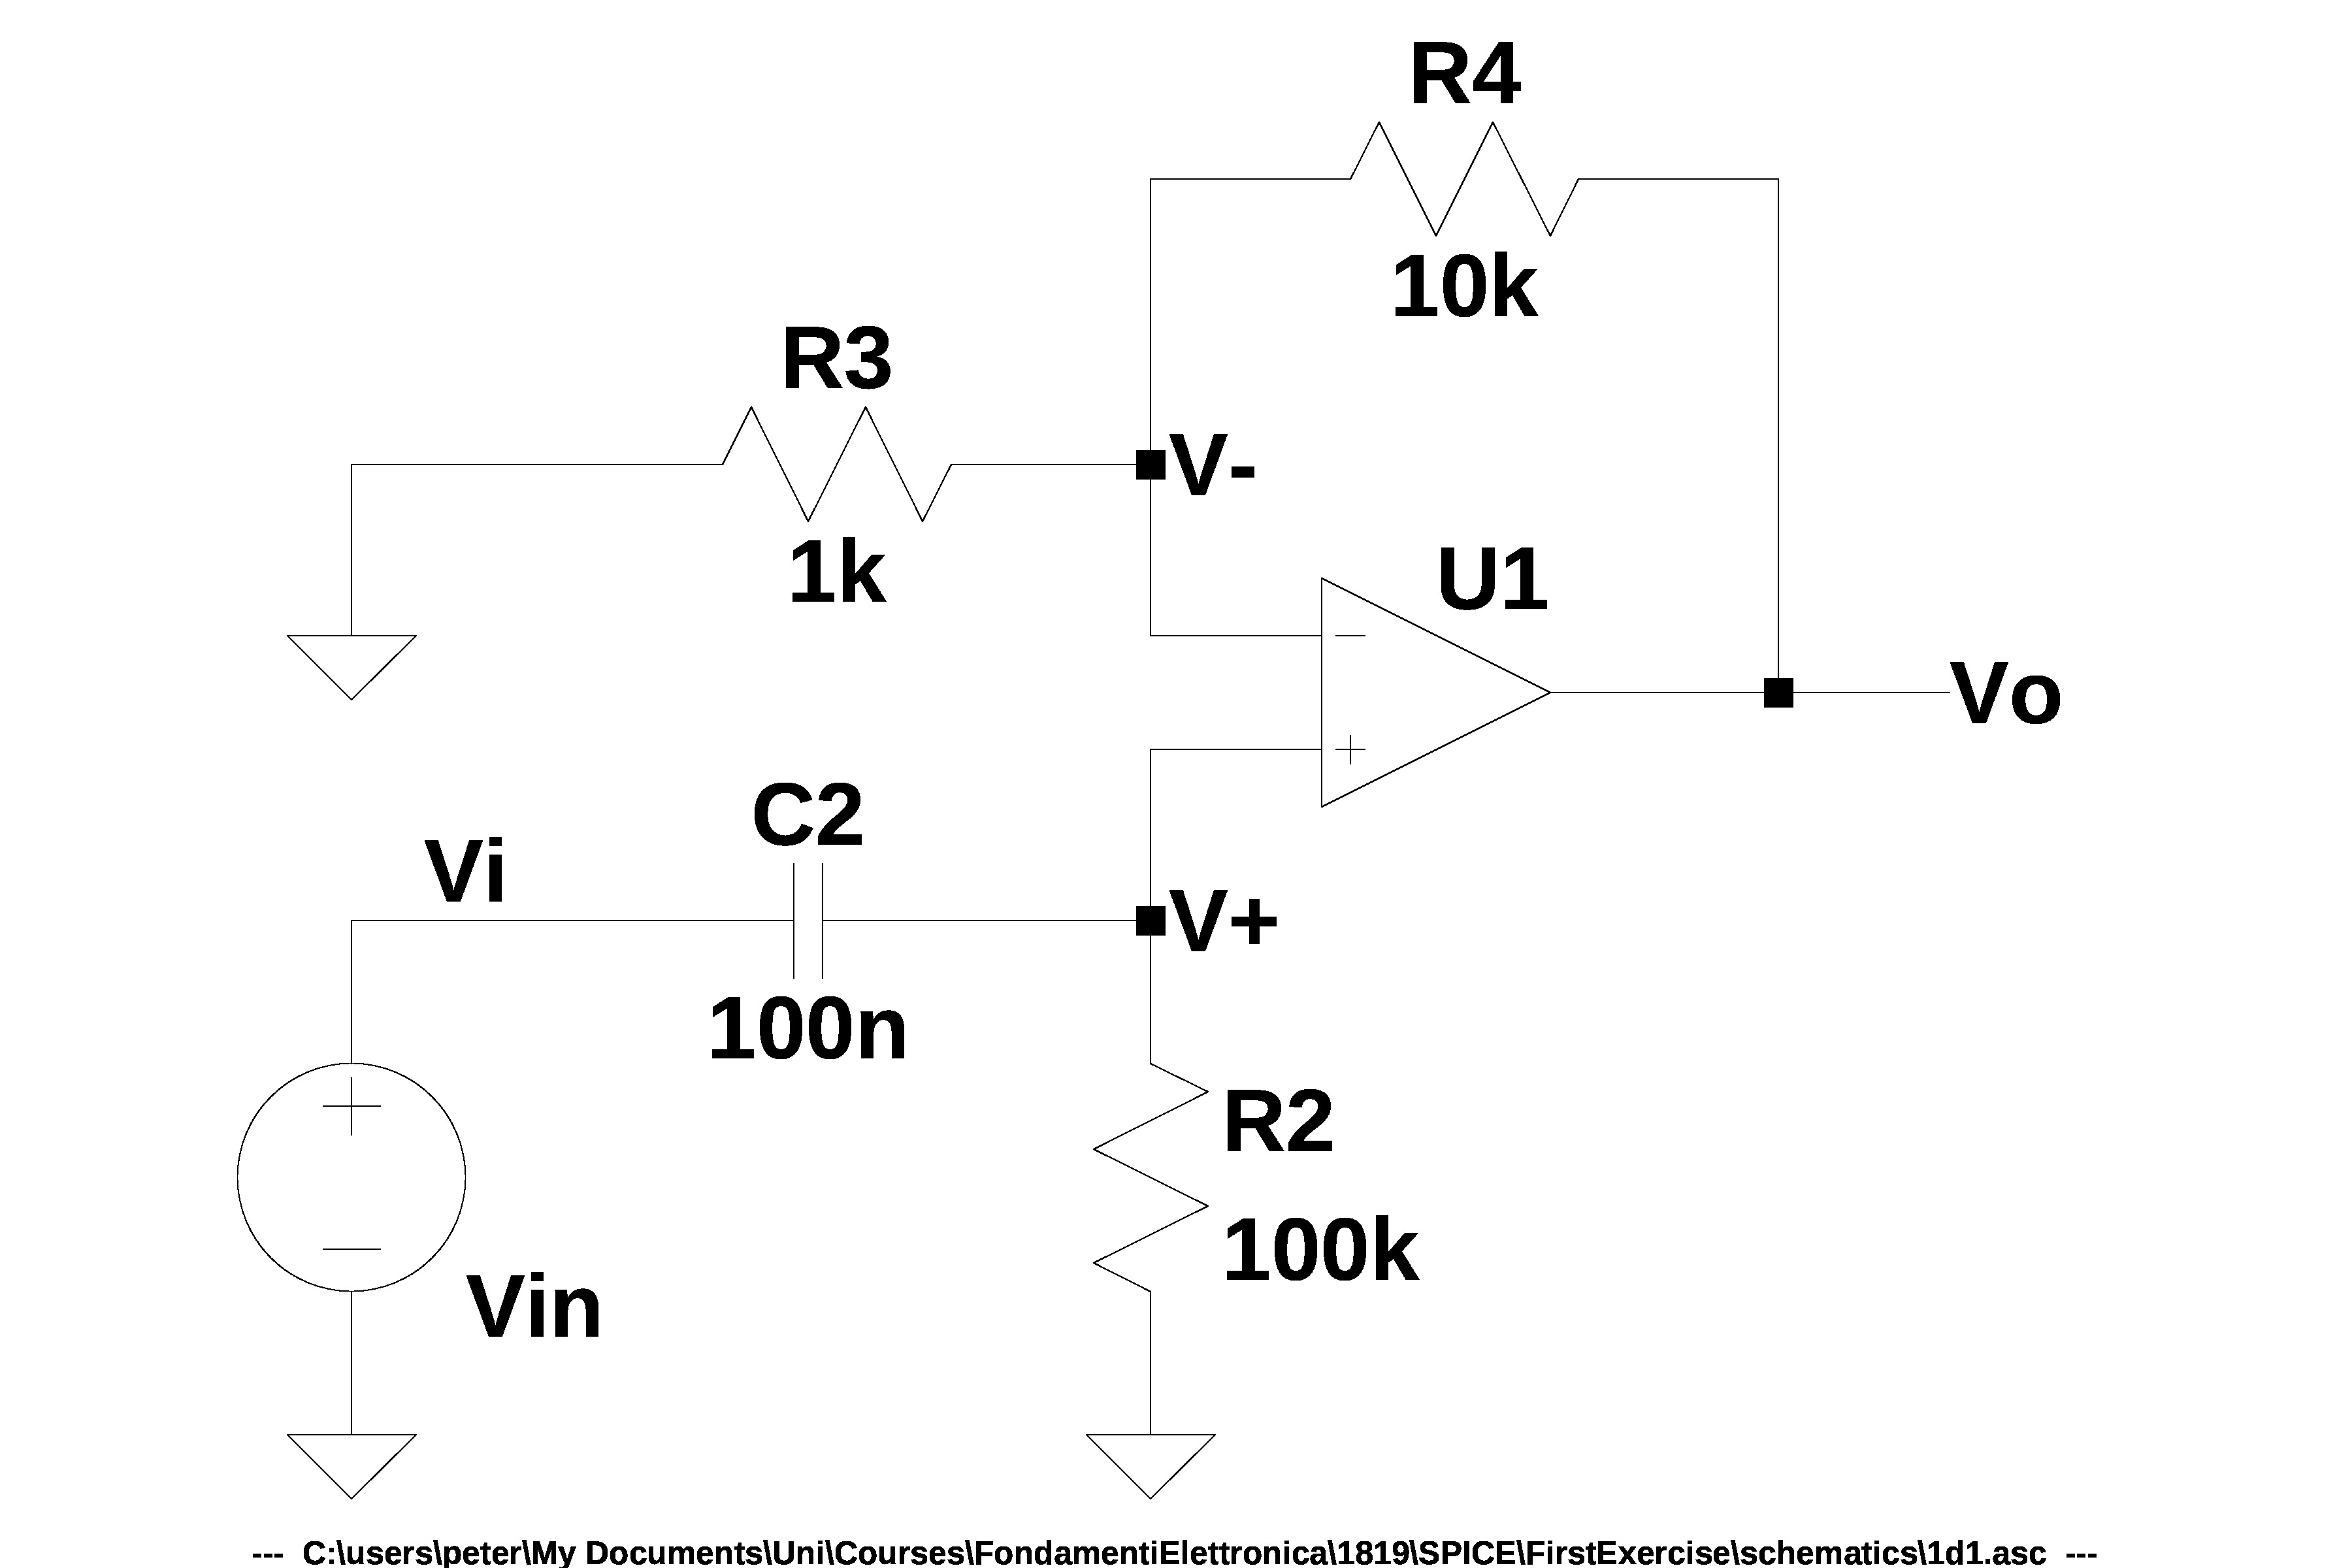
\includegraphics[width=8cm]{schematics/1d1.jpg}
  \caption{Audio amplifier - Ideal op. amp.}
  \label{1d1schematics}
\end{figure}

By the analysis of the figure \ref{1d1schematics}'s circuit, It's possible to calculate the node $V_+$ voltage from the ratio of the voltage divider formed by $R_2$ and $C_2$, indeed the node $V_+$ voltage is the same voltage of the resistance $R_2$ (equation \ref{eq:V_+}).\\
\begin{equation} \label{eq:V_+}
  V_+(s) = V_{in}(s)\frac{R_2}{R_2+\frac{1}{sC_2}} =
  V_{in}(s)\frac{R_2}{R_2+\frac{1}{sC_2}}\frac{sC_2}{sC_2} =
  V_{in}(s)\frac{sC_2R_2}{1+sC_2R_2}
\end{equation}

The negative feedback produces the virtual short circuit effect, so the $V_-$ and the $V_+$ voltages have virtually the same value (equation \ref{eq:V_-}), and, because of the fact that the ideal operational amplifier $U_1$ isn't absorb current from the $V_-$ and the $V_+$ nodes, the current of $I_{R_4}$ is the same current of $I_{R_3}$ (equation \ref{eq:I_R4}).\\
The current $I_{R_3}$ is calculated by the Ohm law (equation \ref{eq:I_R3}).\\

\begin{equation} \label{eq:V_-}
  V_- = V_+
\end{equation}

\begin{equation} \label{eq:I_R4}
  I_{R_4} = I_{R_3}
\end{equation}

\begin{equation} \label{eq:I_R3}
  I_{R_3} = \frac{V_-}{R_3} = \frac{V_+}{R_3}
\end{equation}

By combining the past considerations it's possible to define the output voltage $V_o$ relating to the voltage input $V_{in}$ (equation \ref{eq:V_o}).\\

\begin{equation} \label{eq:V_o}
  V_o(s) = V_+(s) + R_4I_{R_4} = V_+(s) + R_4 I_{R_3} = V_+(s) + R_4 \cdot \frac{V_+(s)}{R_3} =
  V_+(s) \cdot \left(1 + \frac{R_4}{R_3} \right) =
  V_{in}(s)\frac{sC_2R_2}{1+sC_2R_2} \cdot \left(1 + \frac{R_4}{R_3} \right)
\end{equation}

Consequently of the equation \ref{eq:V_o}, the transfer function $V_o(s)/V_{in}(s)$ is described by the equation \ref{eq:TF}.\\

\begin{equation} \label{eq:TF}
  \frac{V_o(s)}{V_{in}(s)} = \frac{sC_2R_2}{1+sC_2R_2}\left(1+\frac{R_4}{R_3}\right)
\end{equation}

Defining $K$ as in the equation \ref{eq:K} and $\omega_1$ as in the equation \ref{eq:omega_1}, the transfer function $V_o(s)/V_{in}(s)$ became in the Bode form (equation \ref{eq:TFBode}).\\

\begin{equation} \label{eq:K}
  K = C_2R_2 \cdot \left(1+\frac{R_4}{R_3}\right)
\end{equation}

\begin{equation} \label{eq:omega_1}
  \omega_1 = \frac{1}{C_2R_2}
\end{equation}

\begin{equation} \label{eq:TFBode}
  \frac{V_o(s)}{V_{in}(s)} = K \frac{s}{1+s\frac{1}{\omega_1}}
\end{equation}

Finally it's possible to calculate the frequency domain by the analysis of the transfer function's Bode form (equations \ref{eq:KdB} and \ref{eq:omega_1log}).\\
\begin{equation} \label{eq:KdB}
  K|_{dB} = 20\log_{10}|K| = \log_{10}\left|C_2R_2 \cdot \left(1+\frac{R_4}{R_3}\right)\right| = -19.1722 dB
\end{equation}

\begin{equation} \label{eq:omega_1log}
  \log_{10} |\omega_1| =
  \log_{10} \left| \frac{1}{C_2R_2} \right|= 2.0000
\end{equation}

\section{Voltage output waveform - LT1028 op. amp.}
\begin{figure}[H]
  \centering
  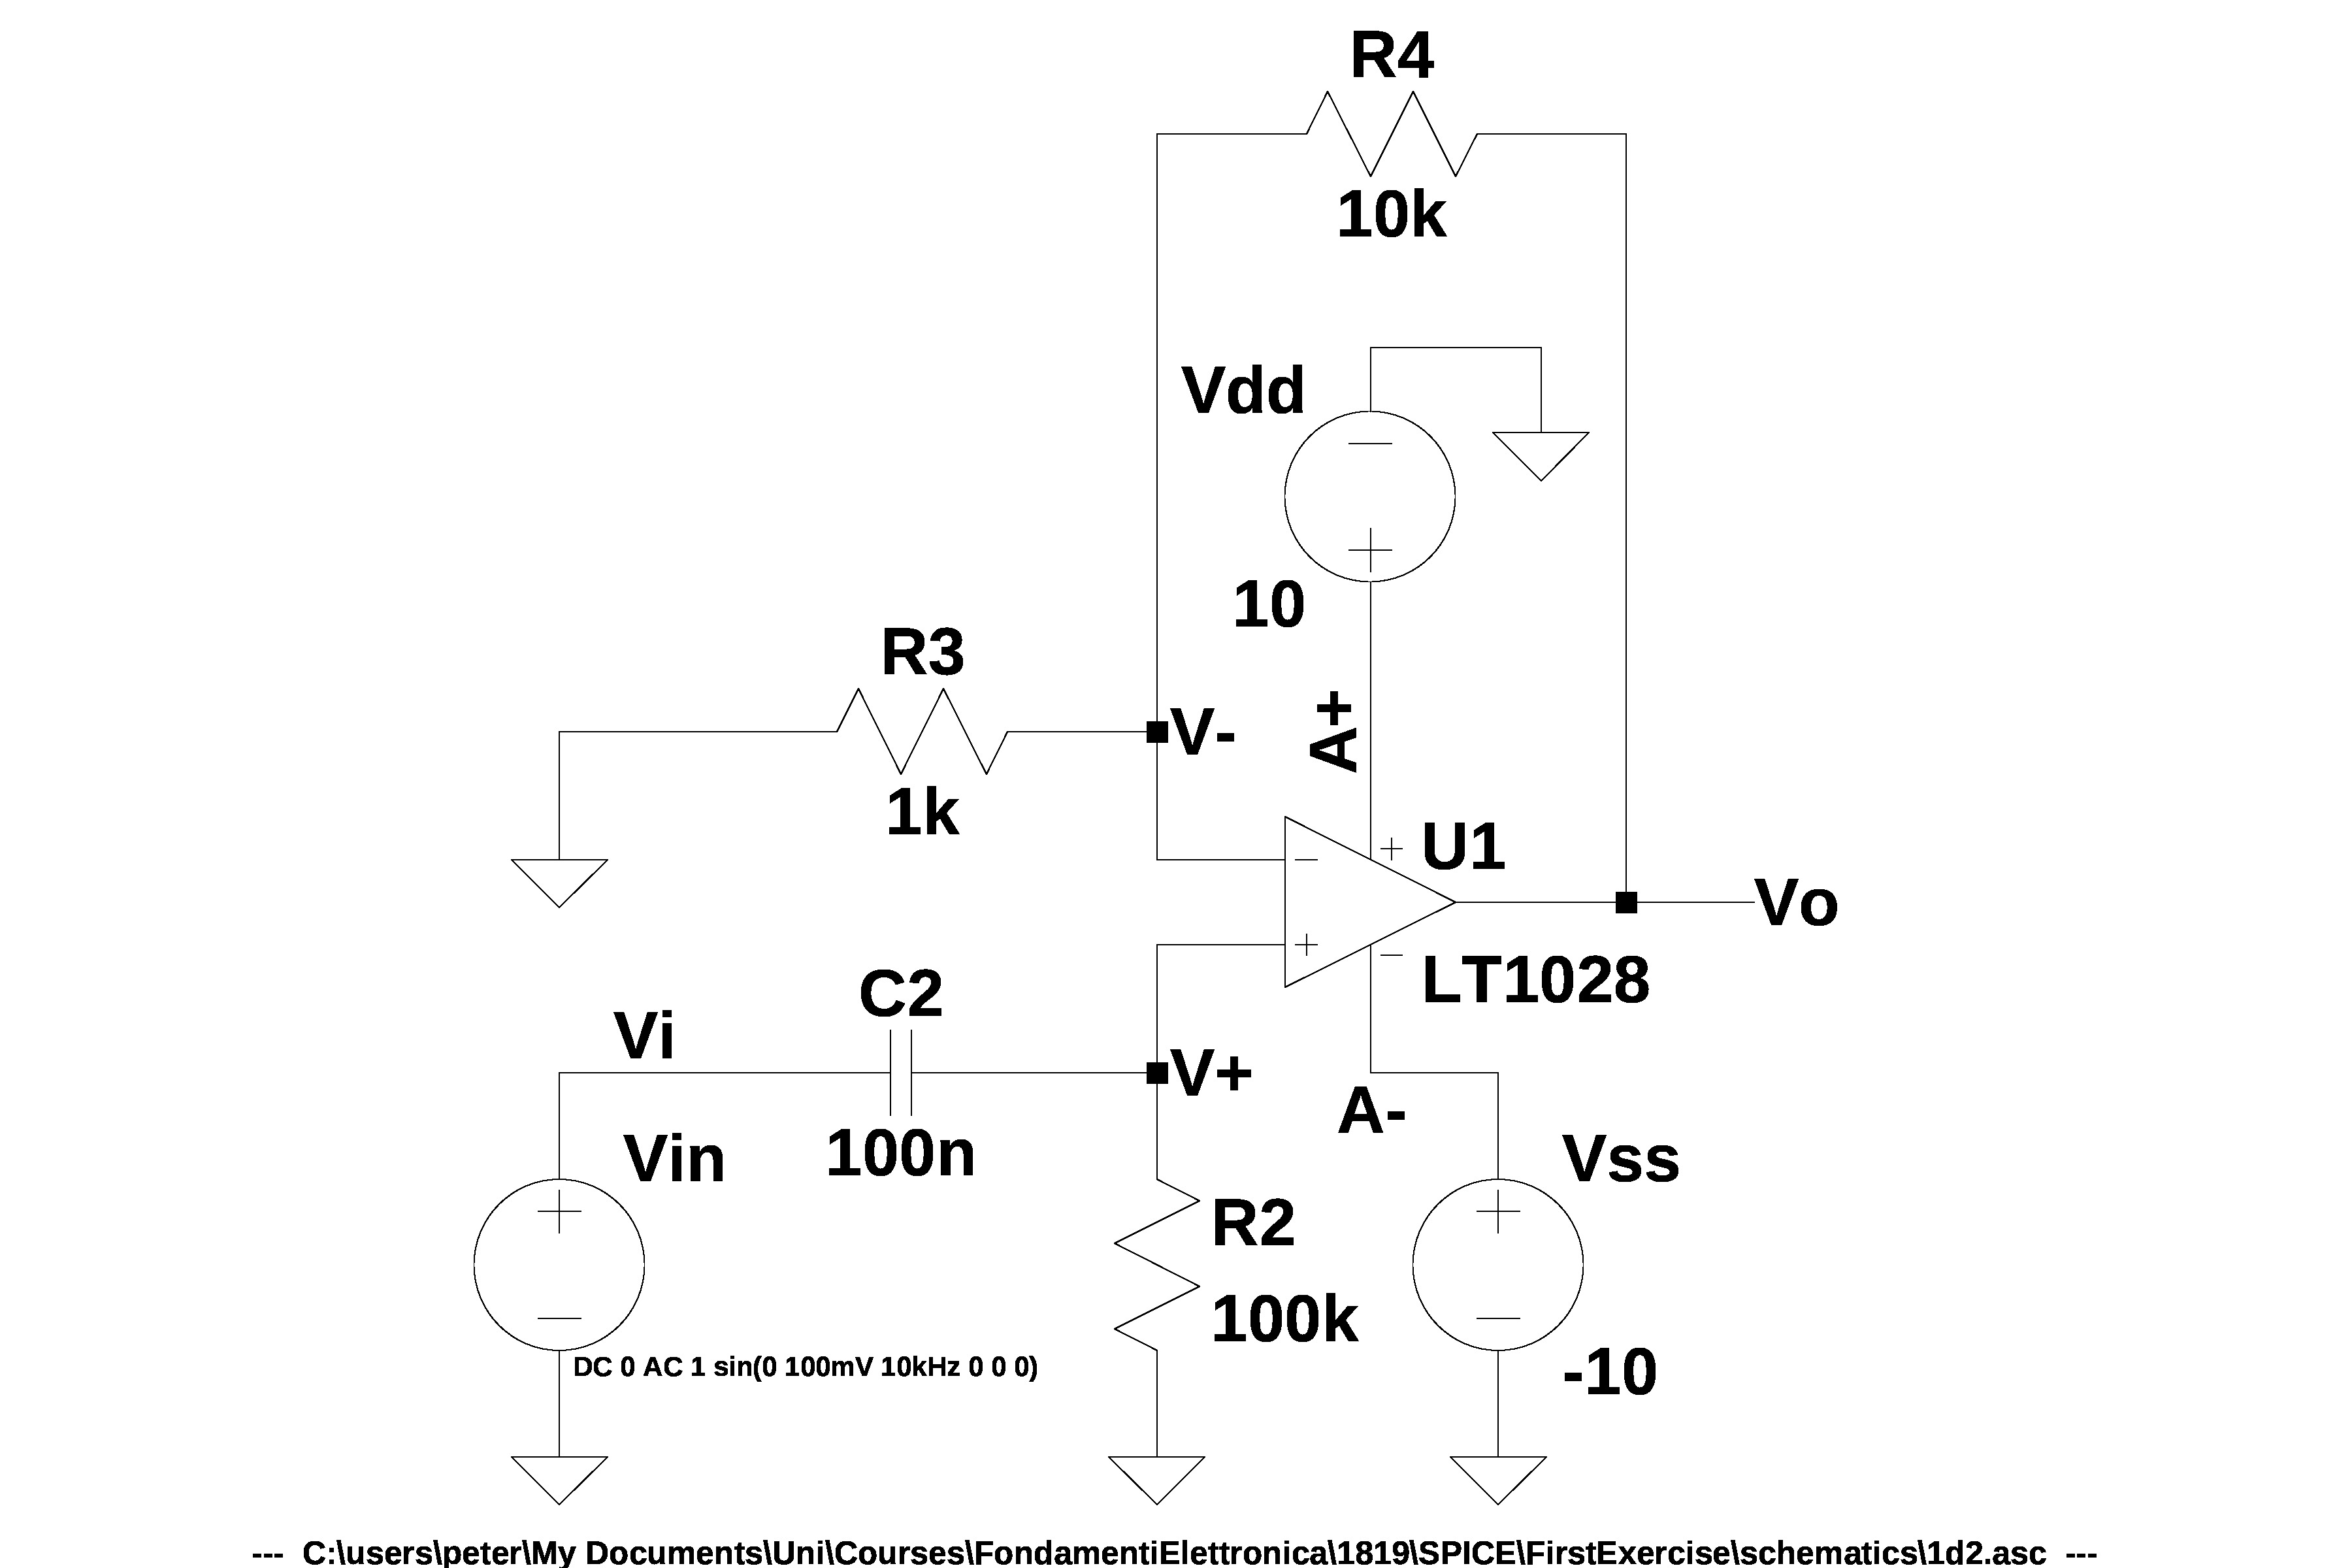
\includegraphics[width=10cm]{schematics/1d2.jpg}
  \caption{Audio amplifier - LT1028 op. amp.}
  \label{1d2schematics}
\end{figure}

From now it's considered the circuit of the figure \ref{1d2schematics}.\par
\medskip
In order to simulate the waveform output voltage with a sinusoidal voltage input $V_{in}$ with an amplitude of $10mV$ and the frequencies of $1Hz$, $10Hz$ and $10kHz$, it's possible to use a SPICE transient analysis.\\

\subsection{Netlist}
It's presented the netlist for the SPICE analysis requested.\\
\lstinputlisting{netlist/1d2.cir}

\subsection{Graph}
This graph is the output of the last netlist presented. There are three curves, one for every frequency analyzed ($1Hz$, $10Hz$ and $10kHz$).\\

\begin{figure}[H]
  \centering
  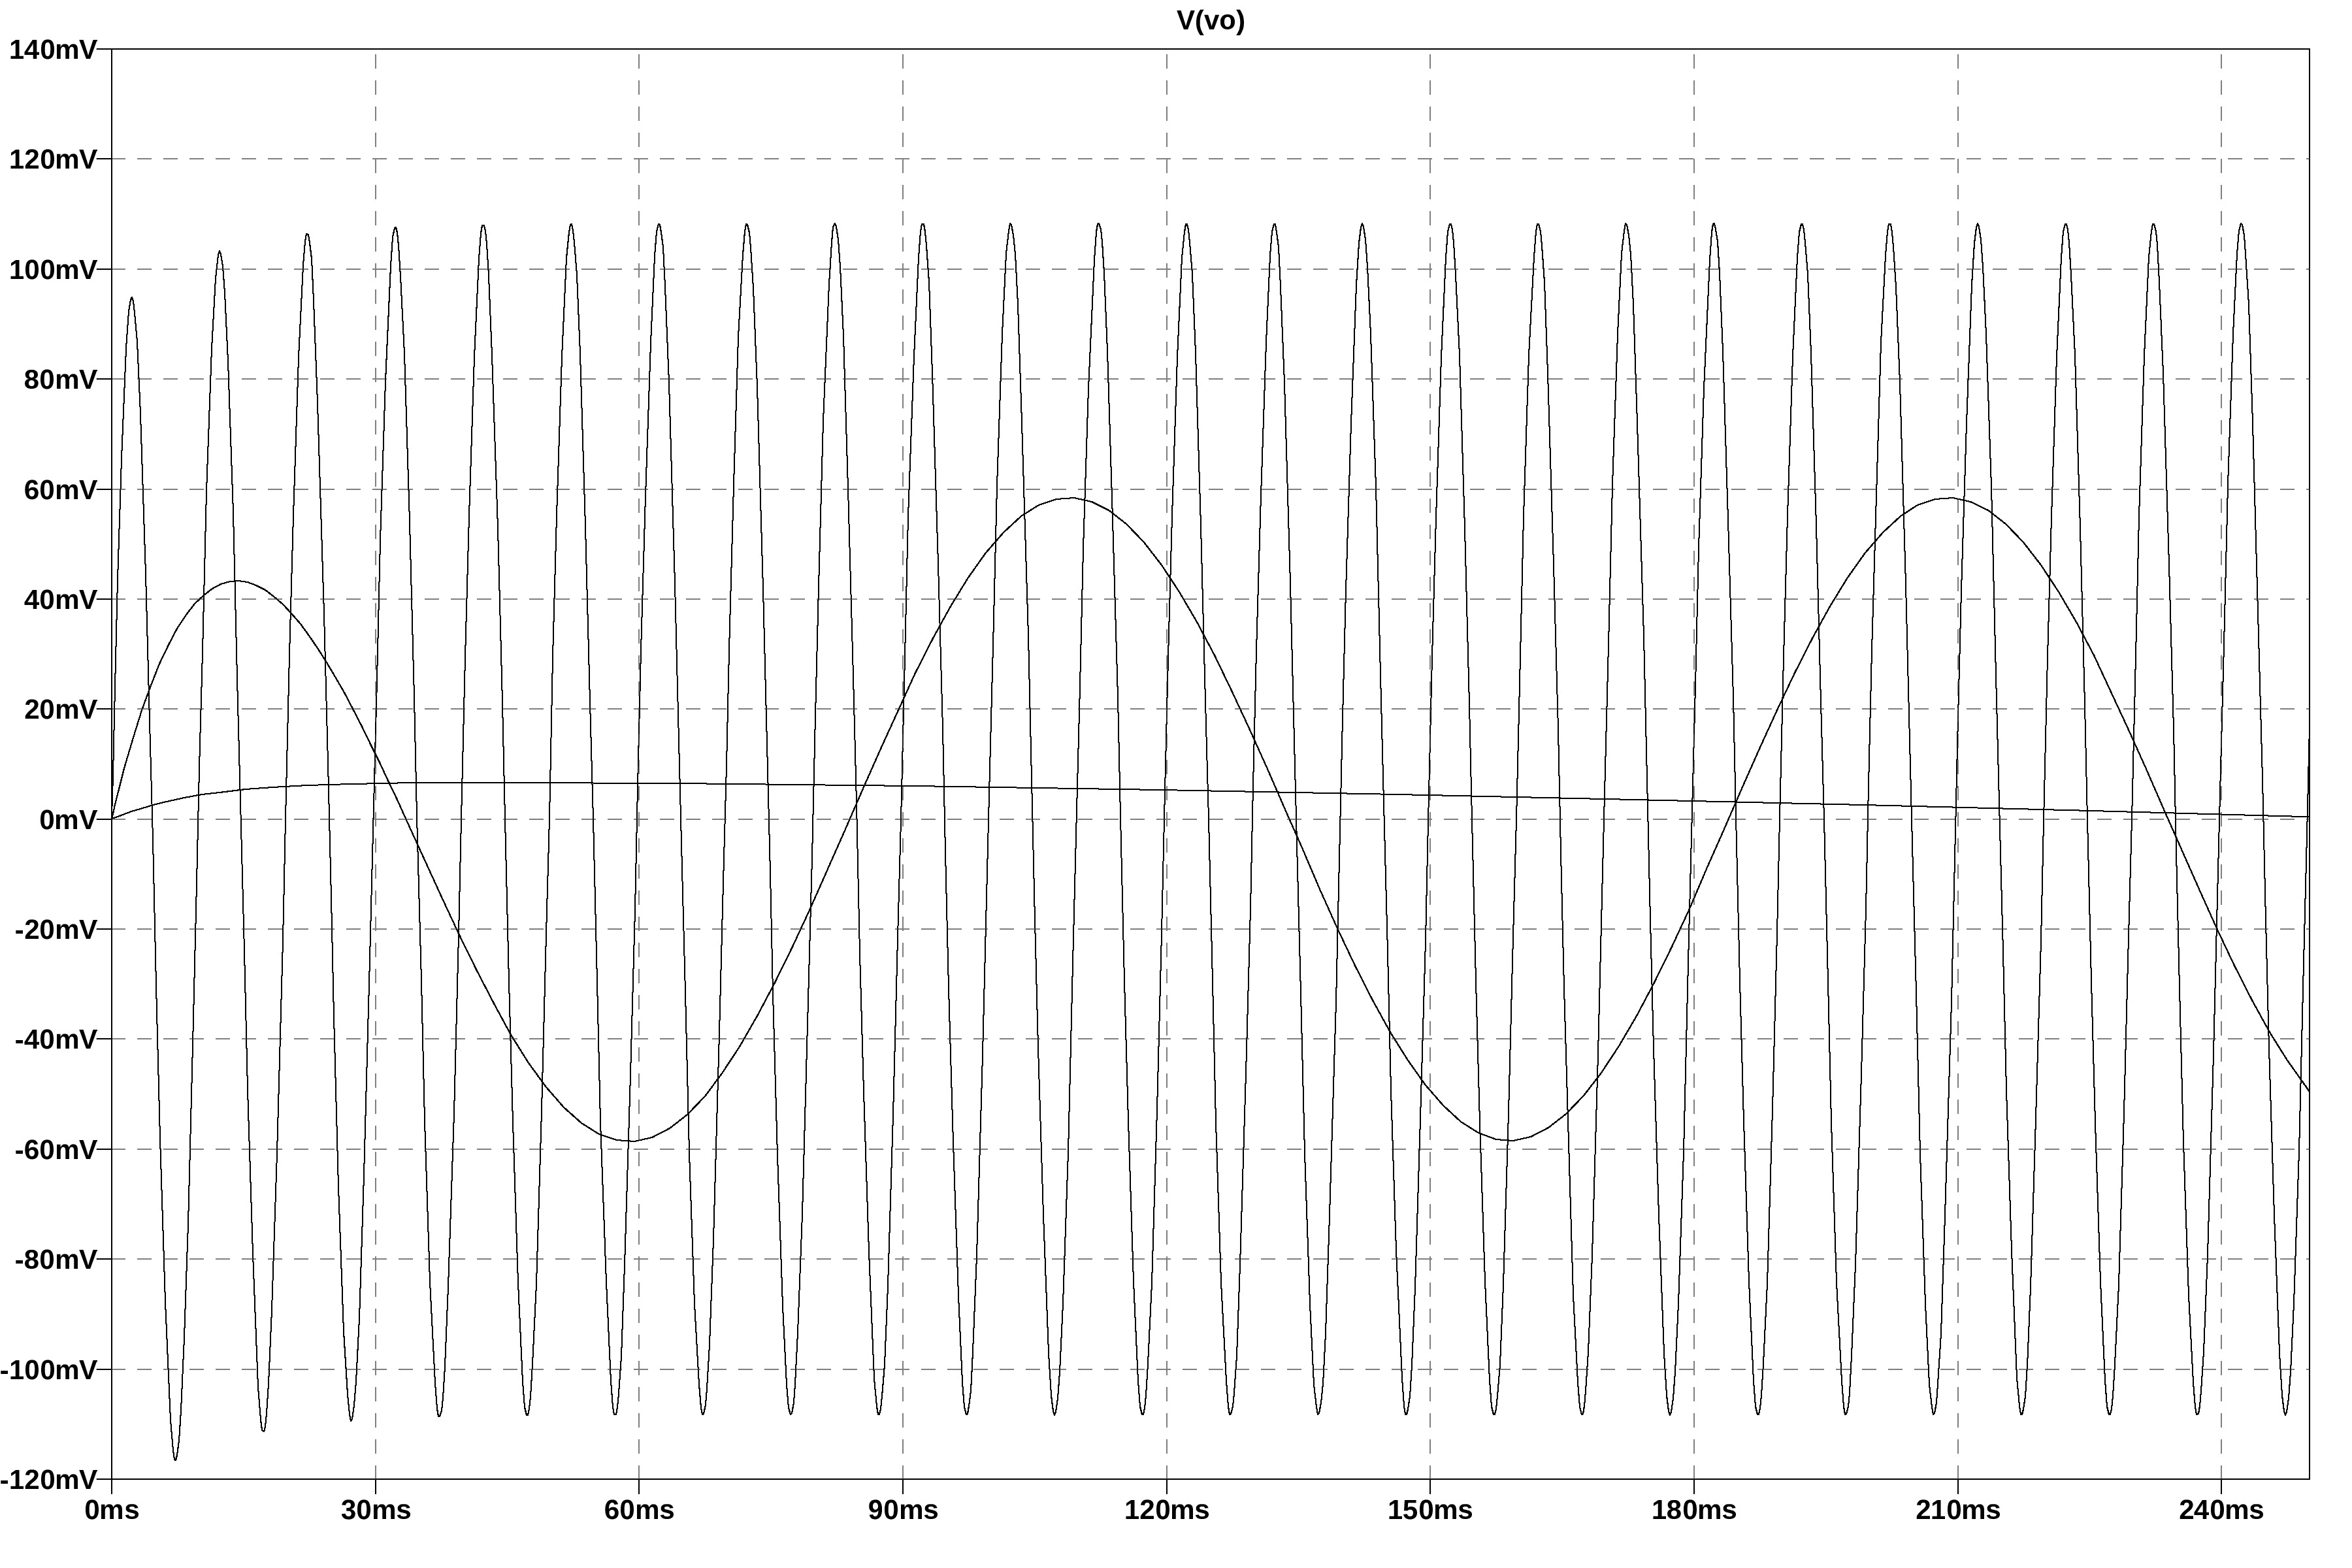
\includegraphics[width=14cm]{graph/1d2.jpg}
  \caption{Audio Amplifier - Voltage output waveform}
  \label{1d2graph}
\end{figure}

\section{Bode plot - LT1028 op. amp.}
The Bode plot could be generated with a SPICE small signal AC analysis.\par

\subsection{Netlist}
It's presented the netlist for the SPICE analysis requested.\\

\lstinputlisting{netlist/1d3.cir}

\subsection{Graph}
The Bode plot generated could be visible in the figure \ref{1d3graph}. The continuous line represents the magnitude and the dashed line represents the phase frequency.\\

\begin{figure}[H]
  \centering
  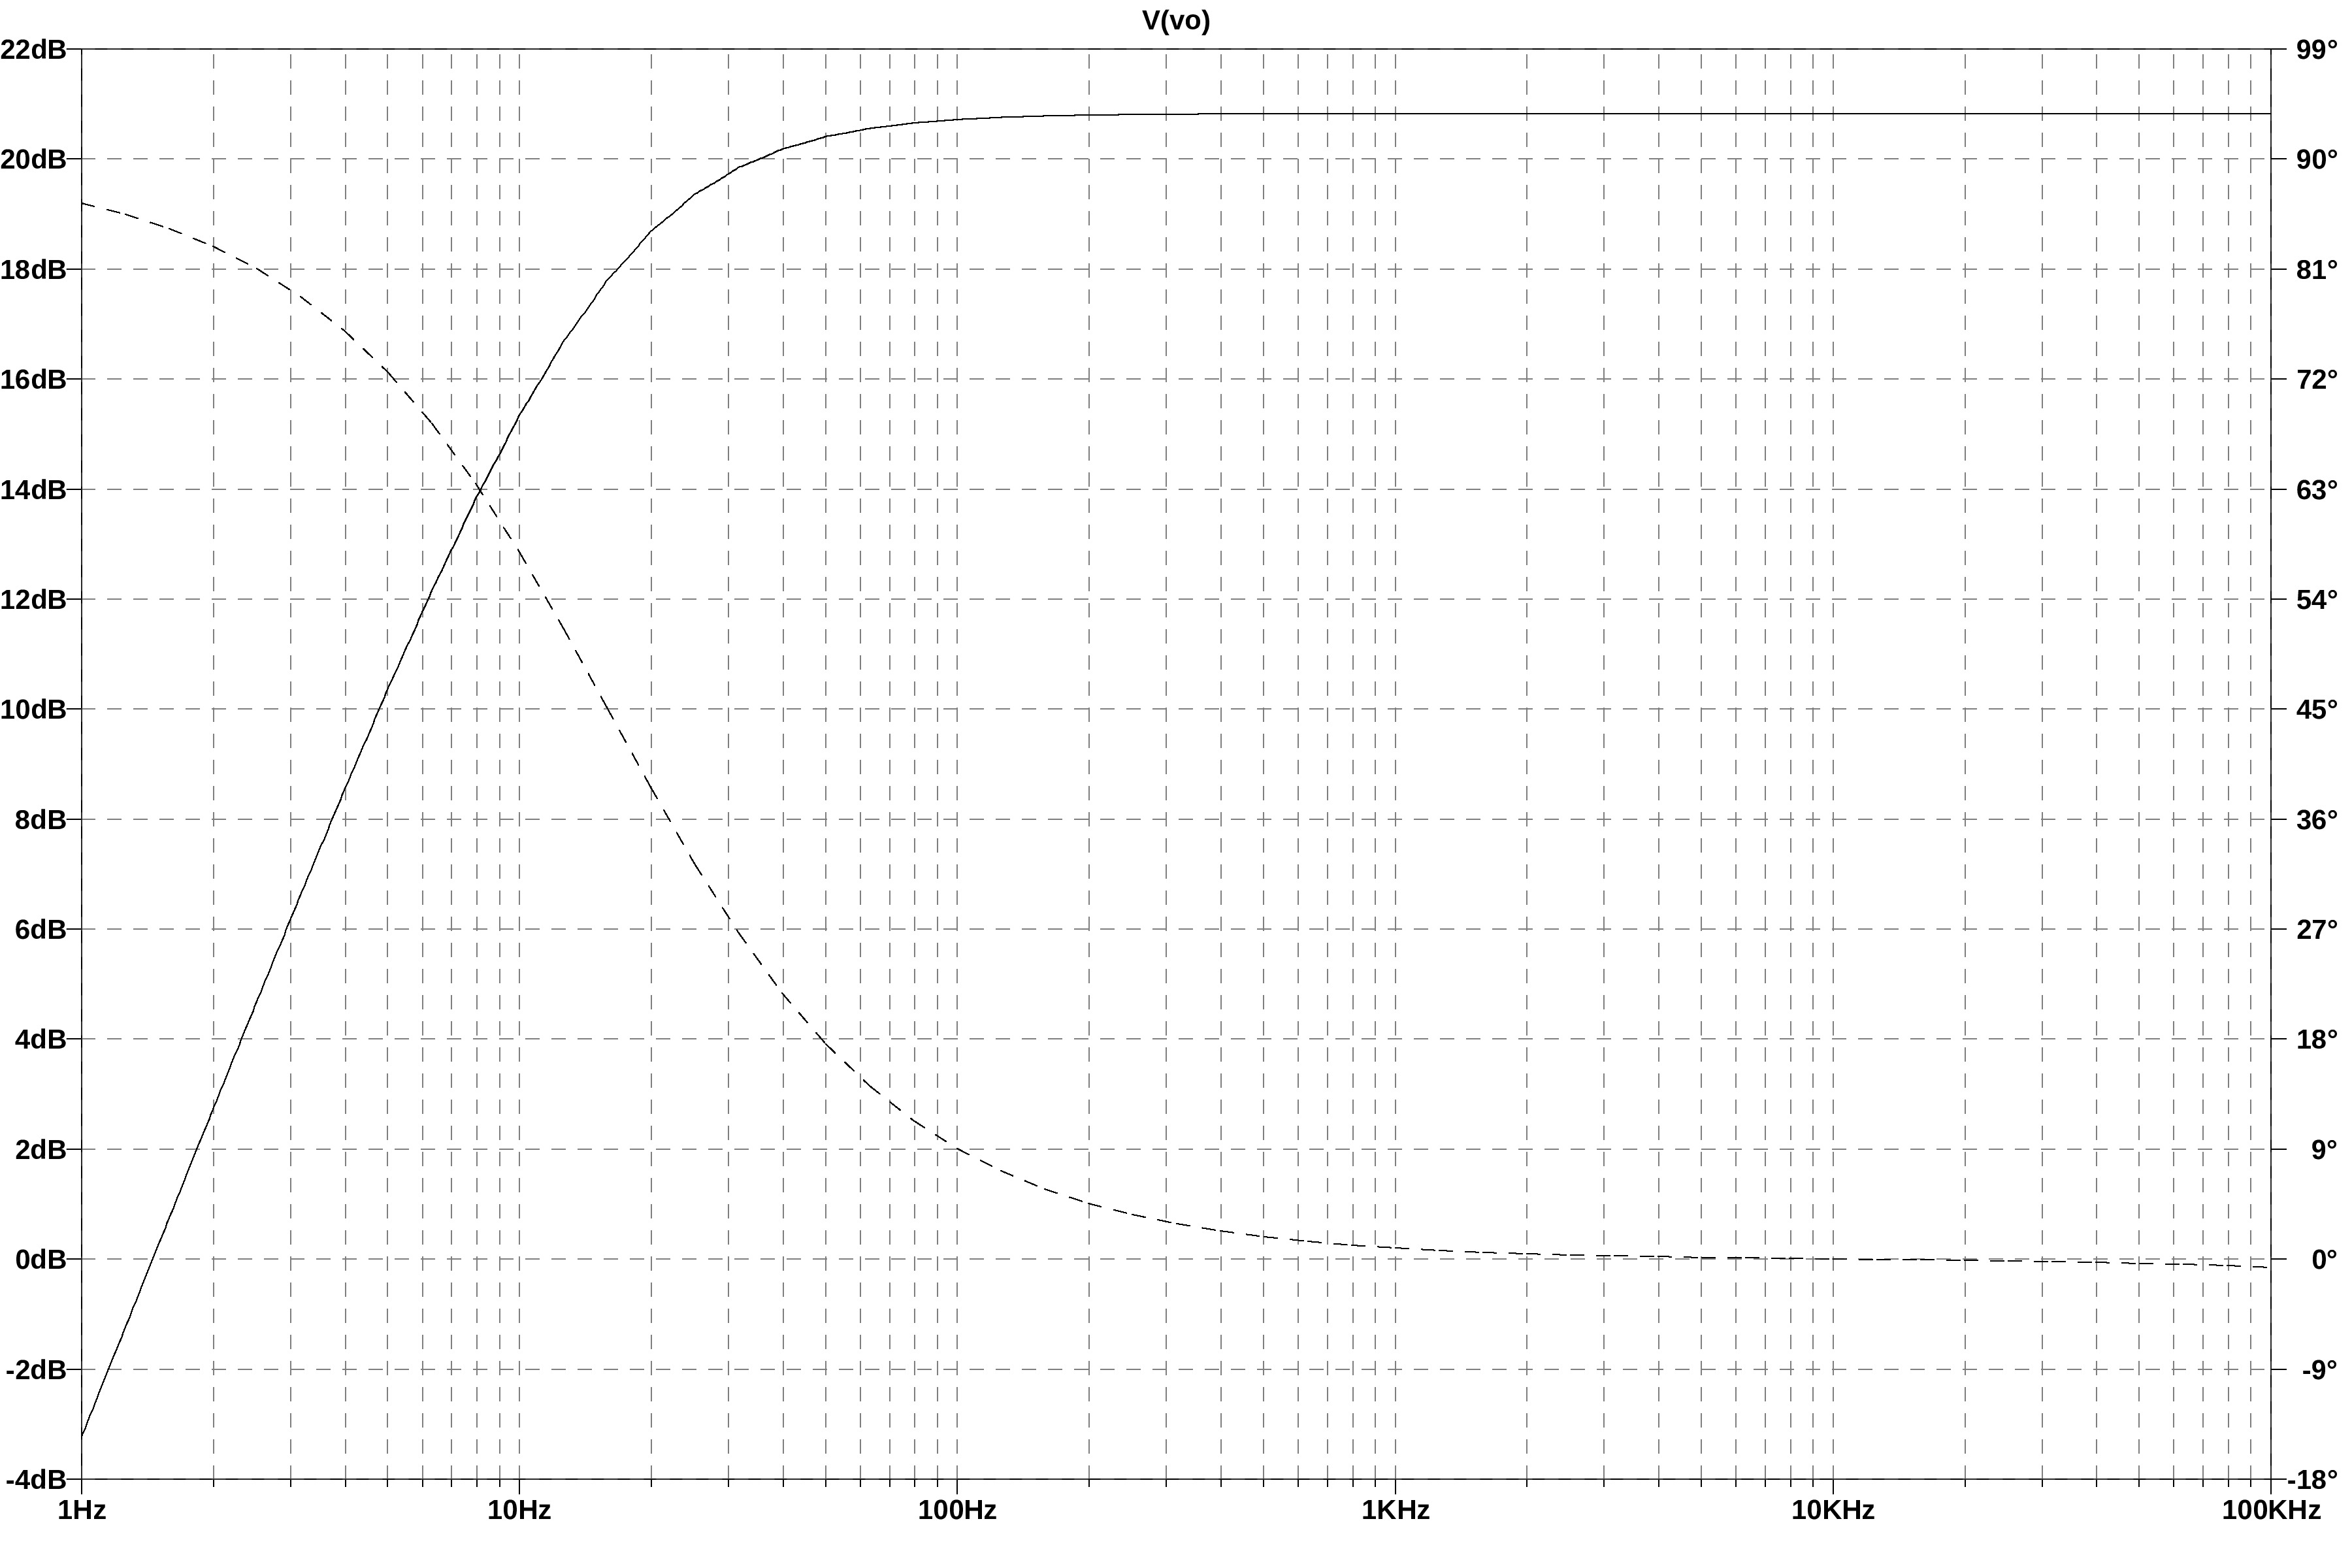
\includegraphics[width=14cm]{graph/1d3.jpg}
  \caption{Audio Amplifier - Bode plot}
  \label{1d3graph}
\end{figure}

\section{Saturation - LT1028 op. amp.}
The voltage output saturation could be analized by giving an abnormally high voltage input to the input.\\
The next netlist analyzes the voltage output with an input with $100V$ amplitude.\\

\lstinputlisting{netlist/1d4.cir}

\begin{figure}[H]
  \centering
  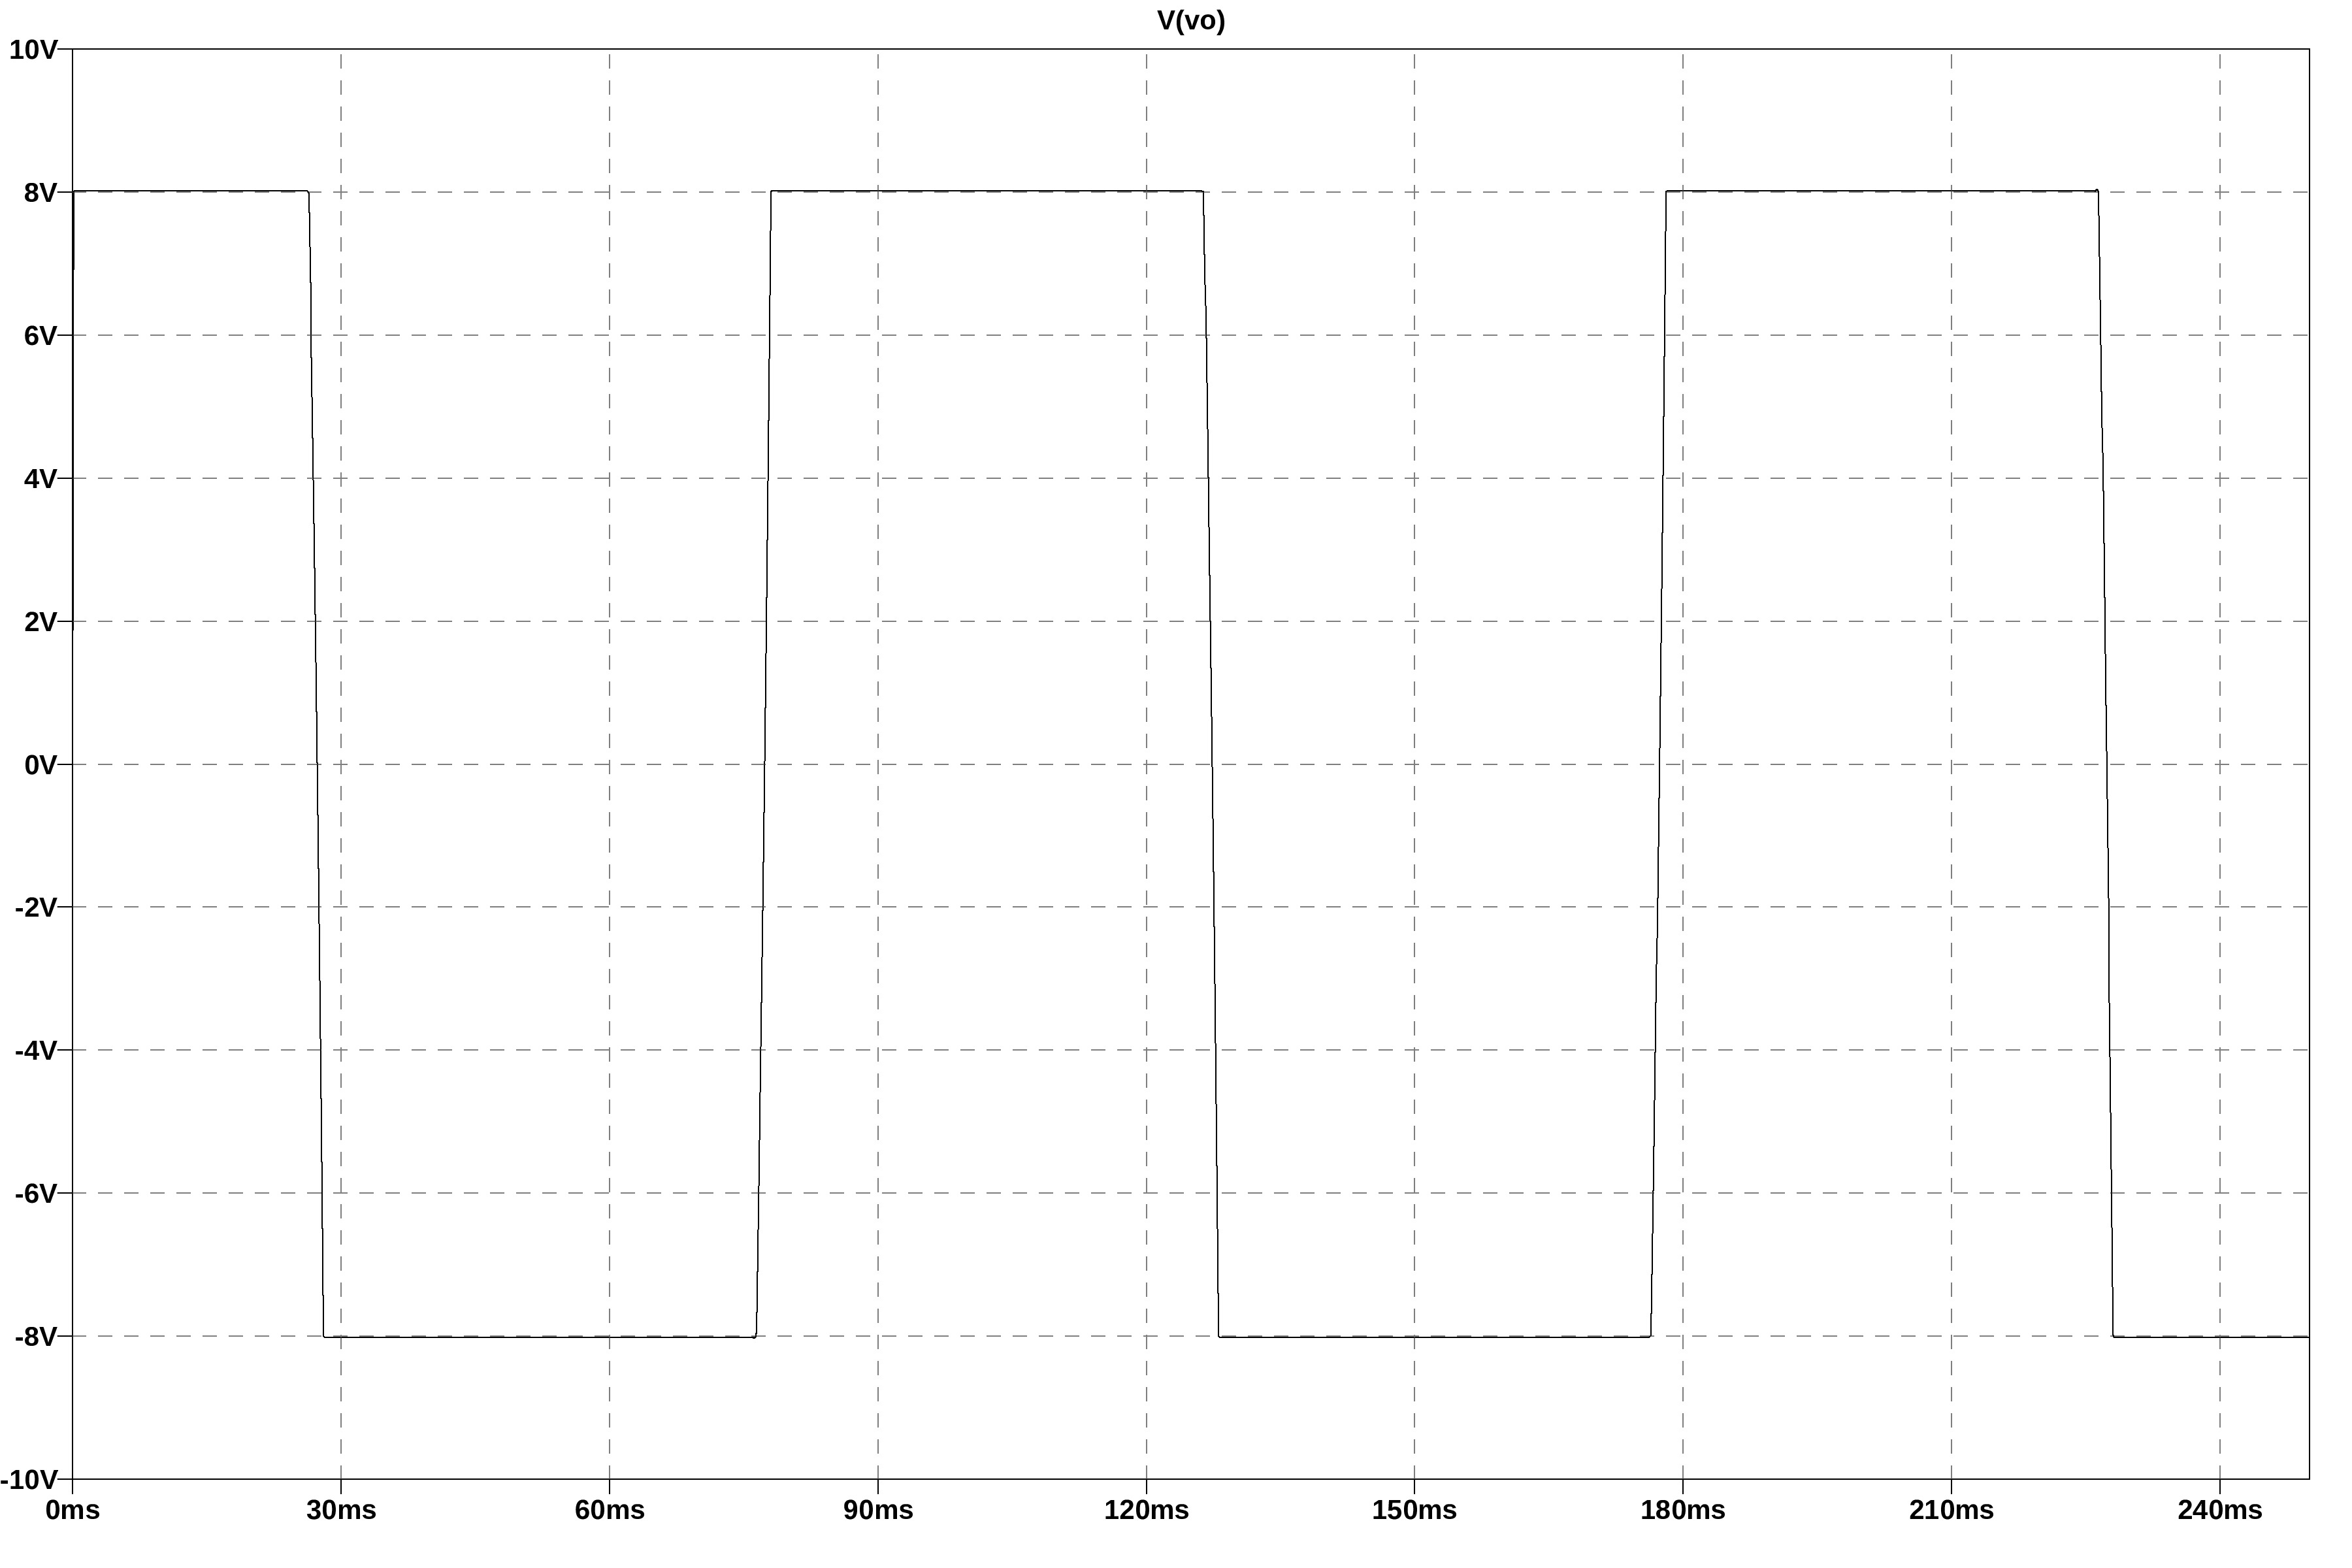
\includegraphics[width=14cm]{graph/1d4.jpg}
  \caption{Audio Amplifier - Output voltage saturation}
  \label{1d4graph}
\end{figure}
The graph generated (figure \ref{1d4graph}) makes clear the fact that the voltage output saturation is on $\pm8V$.\\
So it's possible to calculate wich is the highest input signal that avoids the saturation (equation \ref{eq:V_inSat}).\\

\begin{align}
  |V_o| \leq 8V \nonumber \\
  \left|V_{in}\cdot \frac{j\omega C_2R_2}{1+j\omega C_2R_2} \cdot \left(1 + \frac{R_4}{R_3} \right) \right| \leq 8V \nonumber \\
  |V_{in}|\cdot \left|\frac{j\omega C_2R_2}{1+j\omega C_2R_2} \right| \cdot \left| \left(1 + \frac{R_4}{R_3} \right) \right| \leq 8V \nonumber \\
  |V_{in}|\cdot \frac{\sqrt{(\omega C_2R_2)^2}}{\sqrt{1+(\omega C_2R_2)^2}} \cdot \frac{R_3 + R_4}{R_3} \leq 8V \nonumber \\
  |V_{in}| \leq 8V \cdot \frac{\sqrt{1+(\omega C_2R_2)^2}}{\omega C_2R_2} \cdot \frac{R_3}{R_3 + R_4} \label{eq:V_inSat}
\end{align}

In order to have a maximum value of the input voltage $V_{in}$, the $\omega$ could be setted to a static value.\\
For example with $\omega = 10Hz \cdot 2\pi$ the maximum value of the input voltage is $|V_{in}| \leq 1.36701V$ (output voltage graph on figure \ref{1d4bgraph}).

\begin{figure}[H]
  \centering
  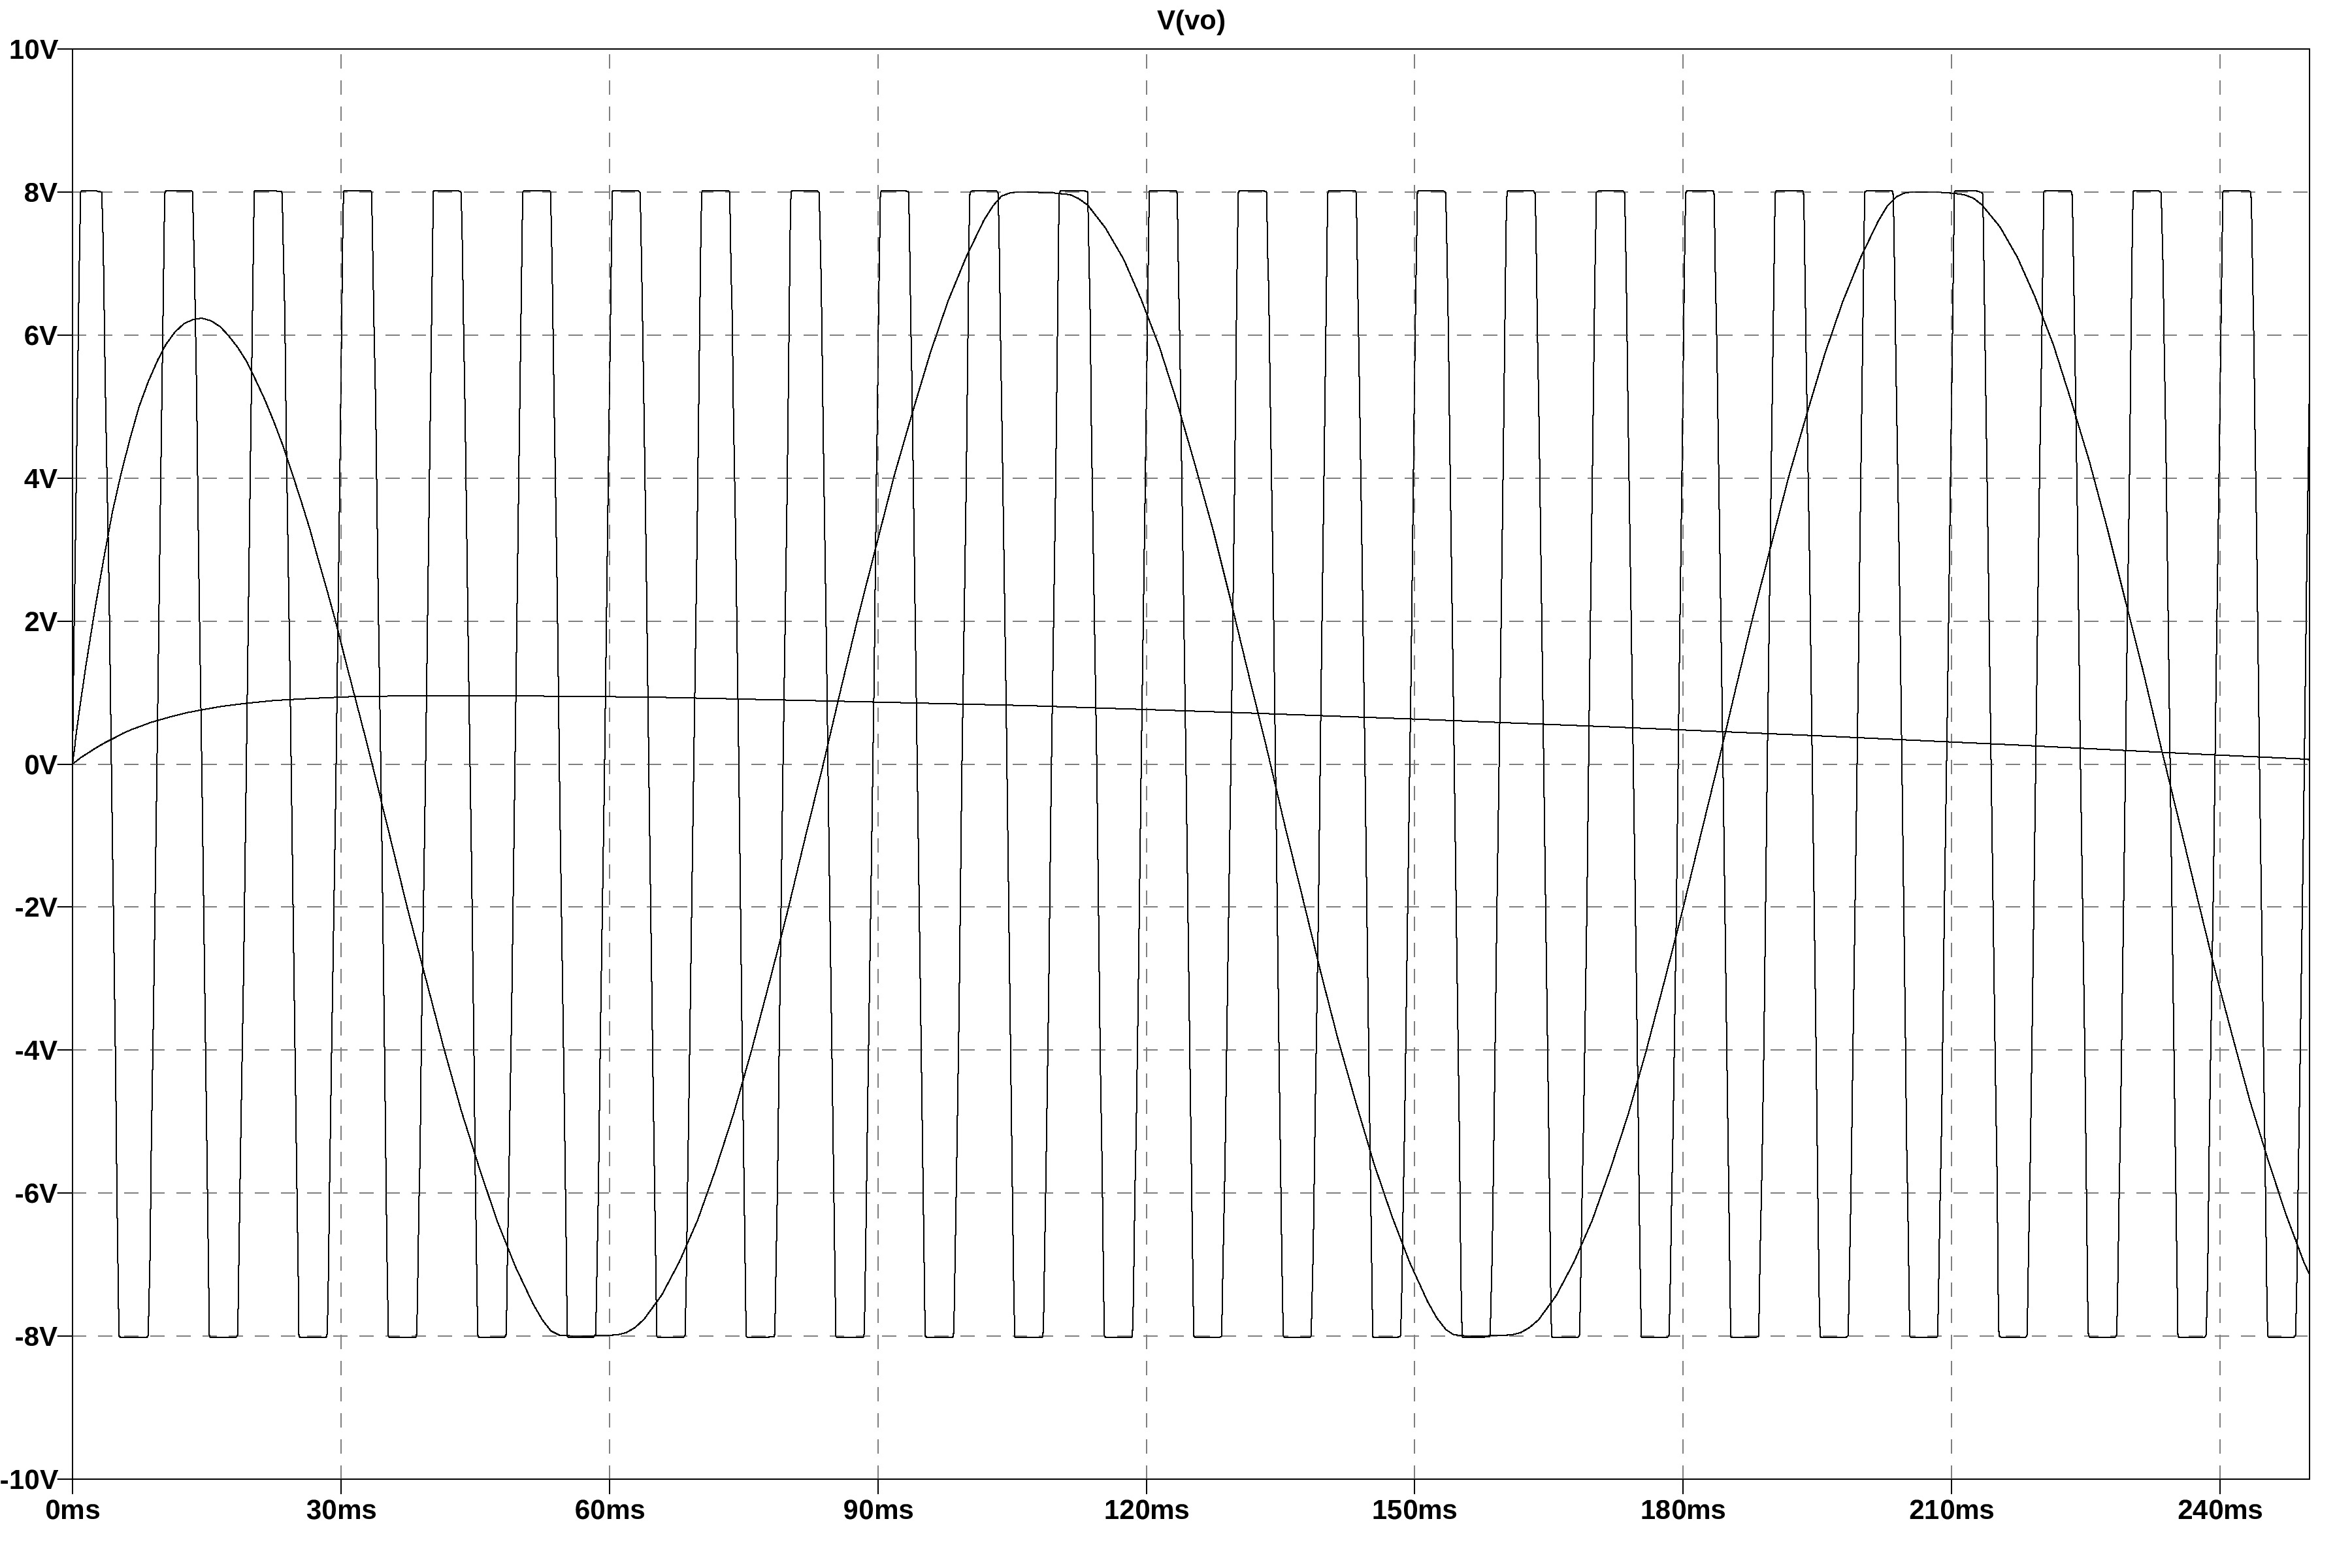
\includegraphics[width=14cm]{graph/1d4b.jpg}
  \caption{Audio Amplifier - Output voltage with an amplitude of the imput voltage equal to $1.36701V$, frequency equal to $10Hz$}
  \label{1d4bgraph}
\end{figure}

\subsection{Output voltage waveform - $V_{in} = 2 \cdot |V_{in MAX} |$}
The netlist used for plot the output voltage waveform with a double input voltage relatively to the maximum input voltage calculated is:\\
\lstinputlisting{netlist/1d4c.cir}

\begin{figure}[H]
  \centering
  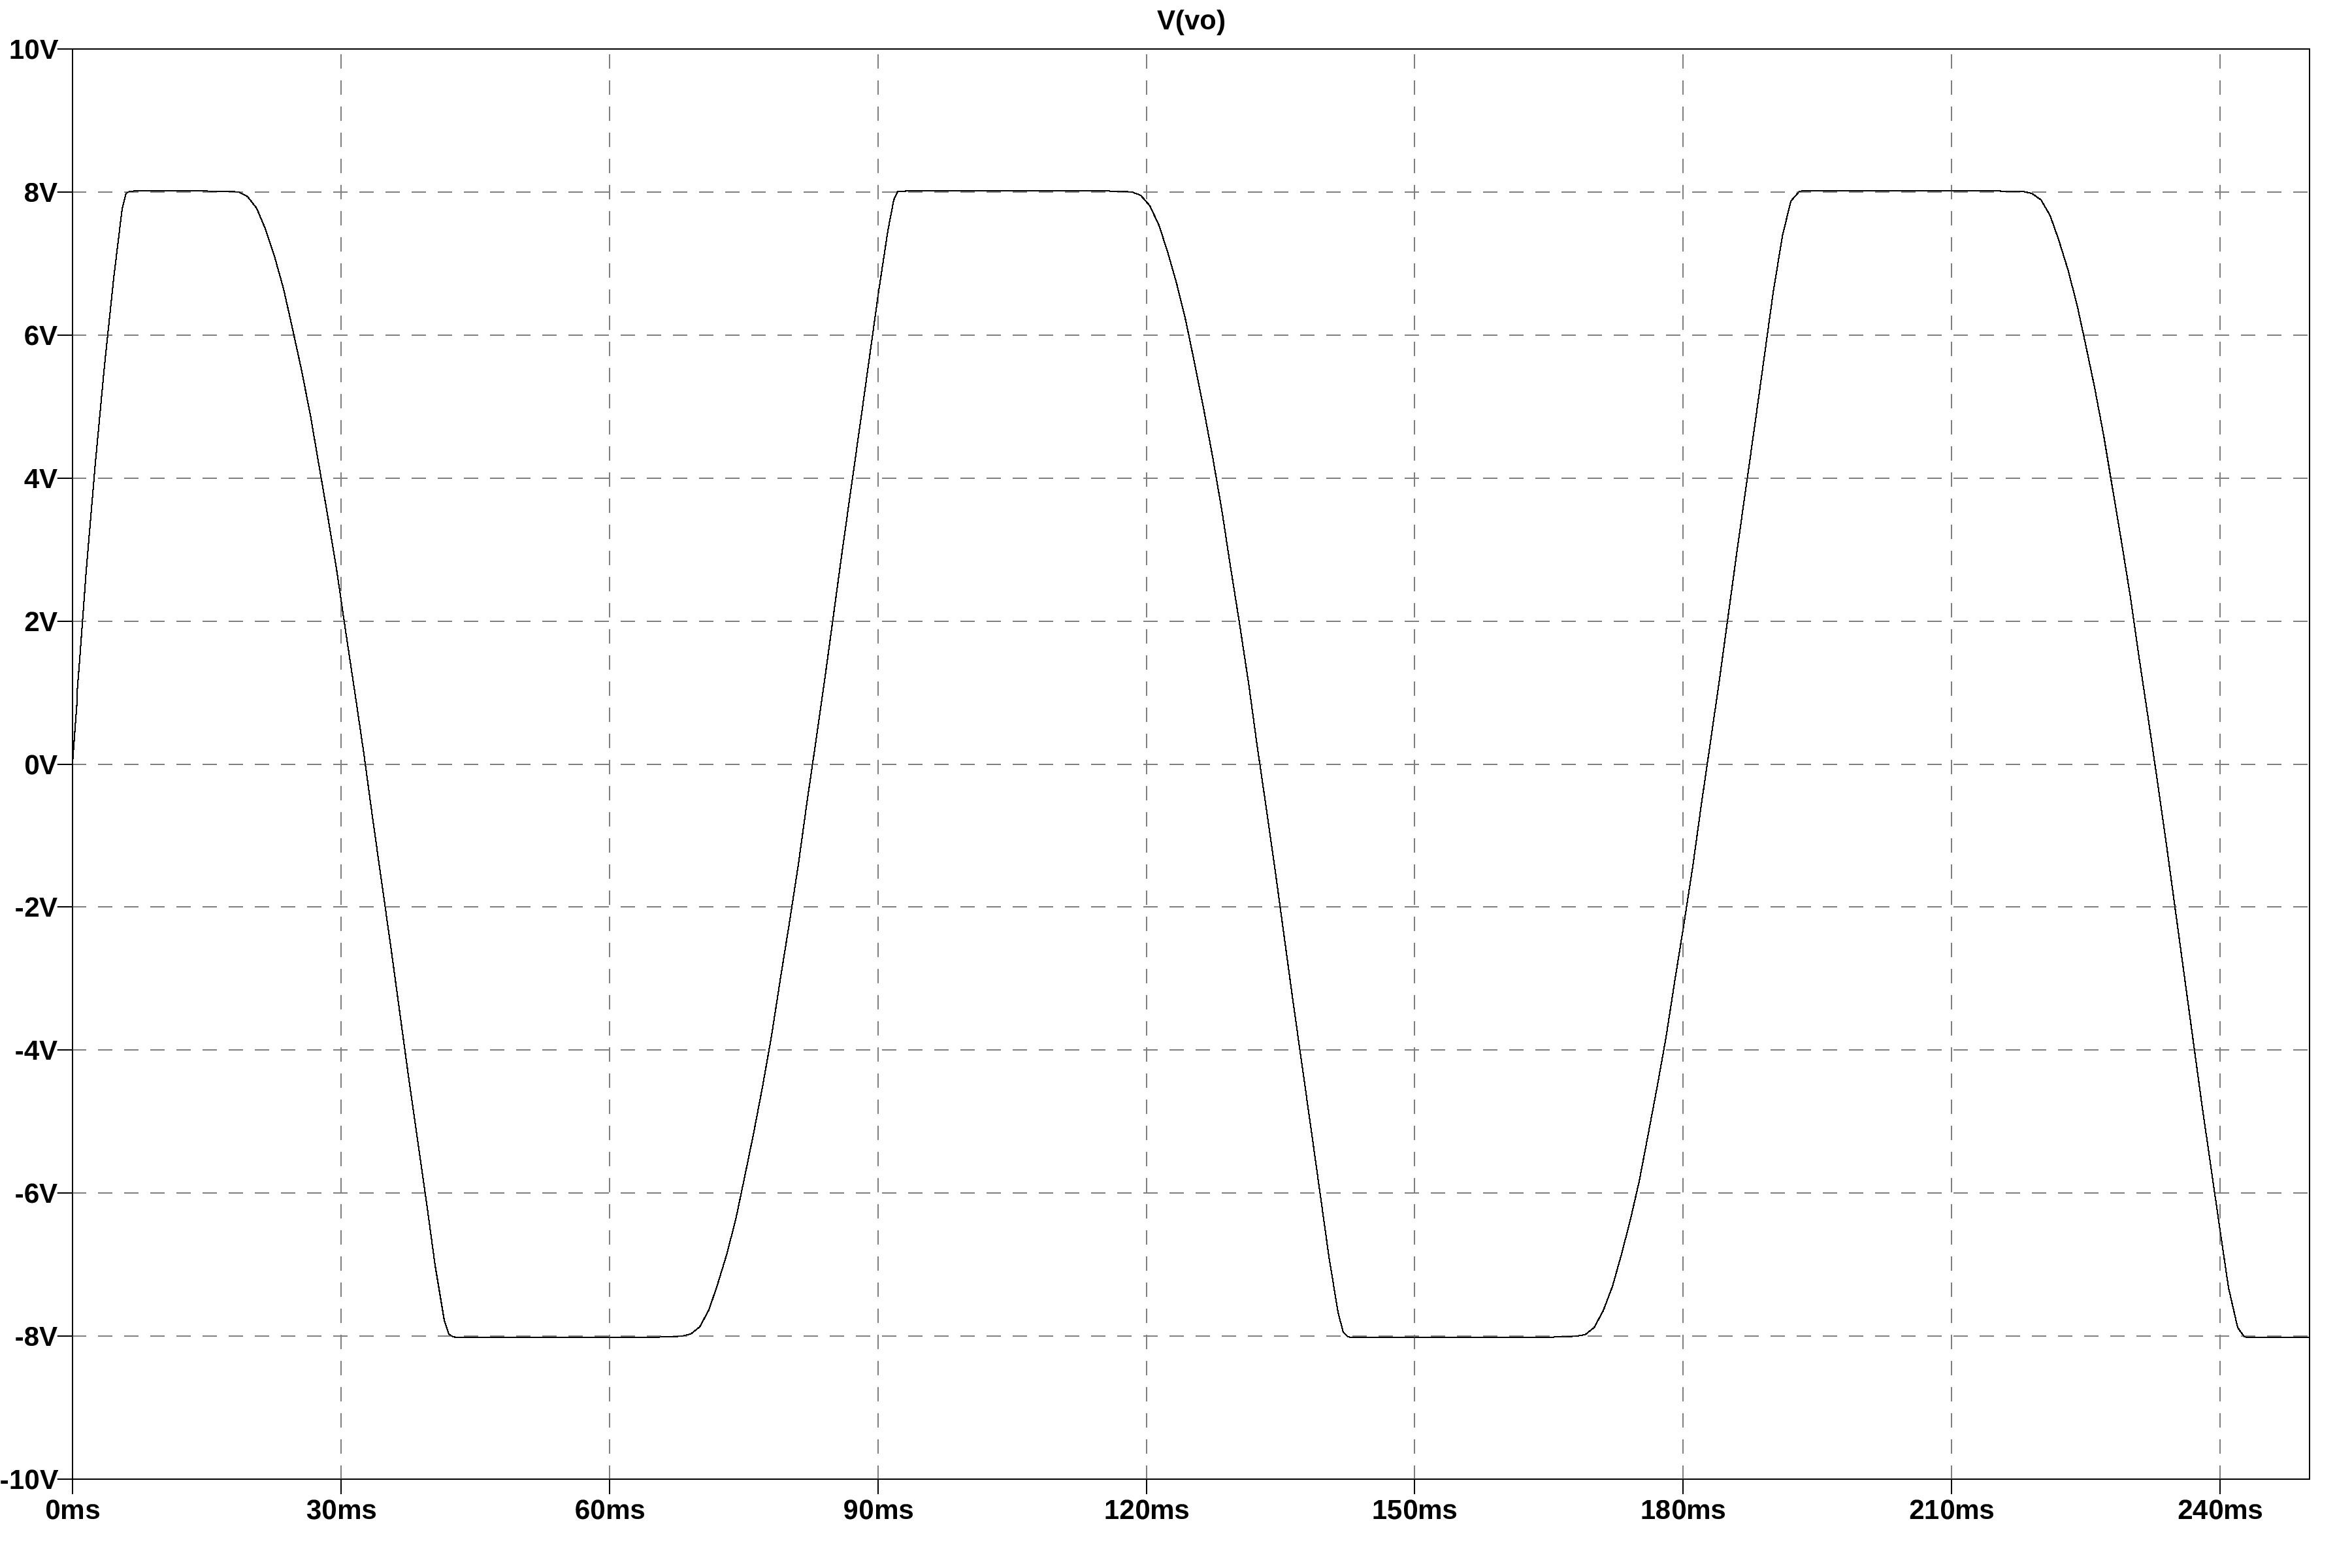
\includegraphics[width=14cm]{graph/1d4c.jpg}
  \caption{Audio Amplifier - Output voltage with an amplitude of the imput voltage equal to $2 \cdot 1.36701V$, frequency equal to $10Hz$}
  \label{1d4cgraph}
\end{figure}

The graph generated is presented on the figure \ref{1d4cgraph}.\\

\section{Saturation - LT1028 op. amp. - $R_2 = 109775.2\Omega$}
Using the equation \ref{eq:V_inSat} and setting $\omega = 10Hz \cdot 2\pi$ the maximum value of the input voltage is $|V_{in}| \leq 1.28091V$ (output voltage graph on figure \ref{1d5graph})

\begin{figure}[H]
  \centering
  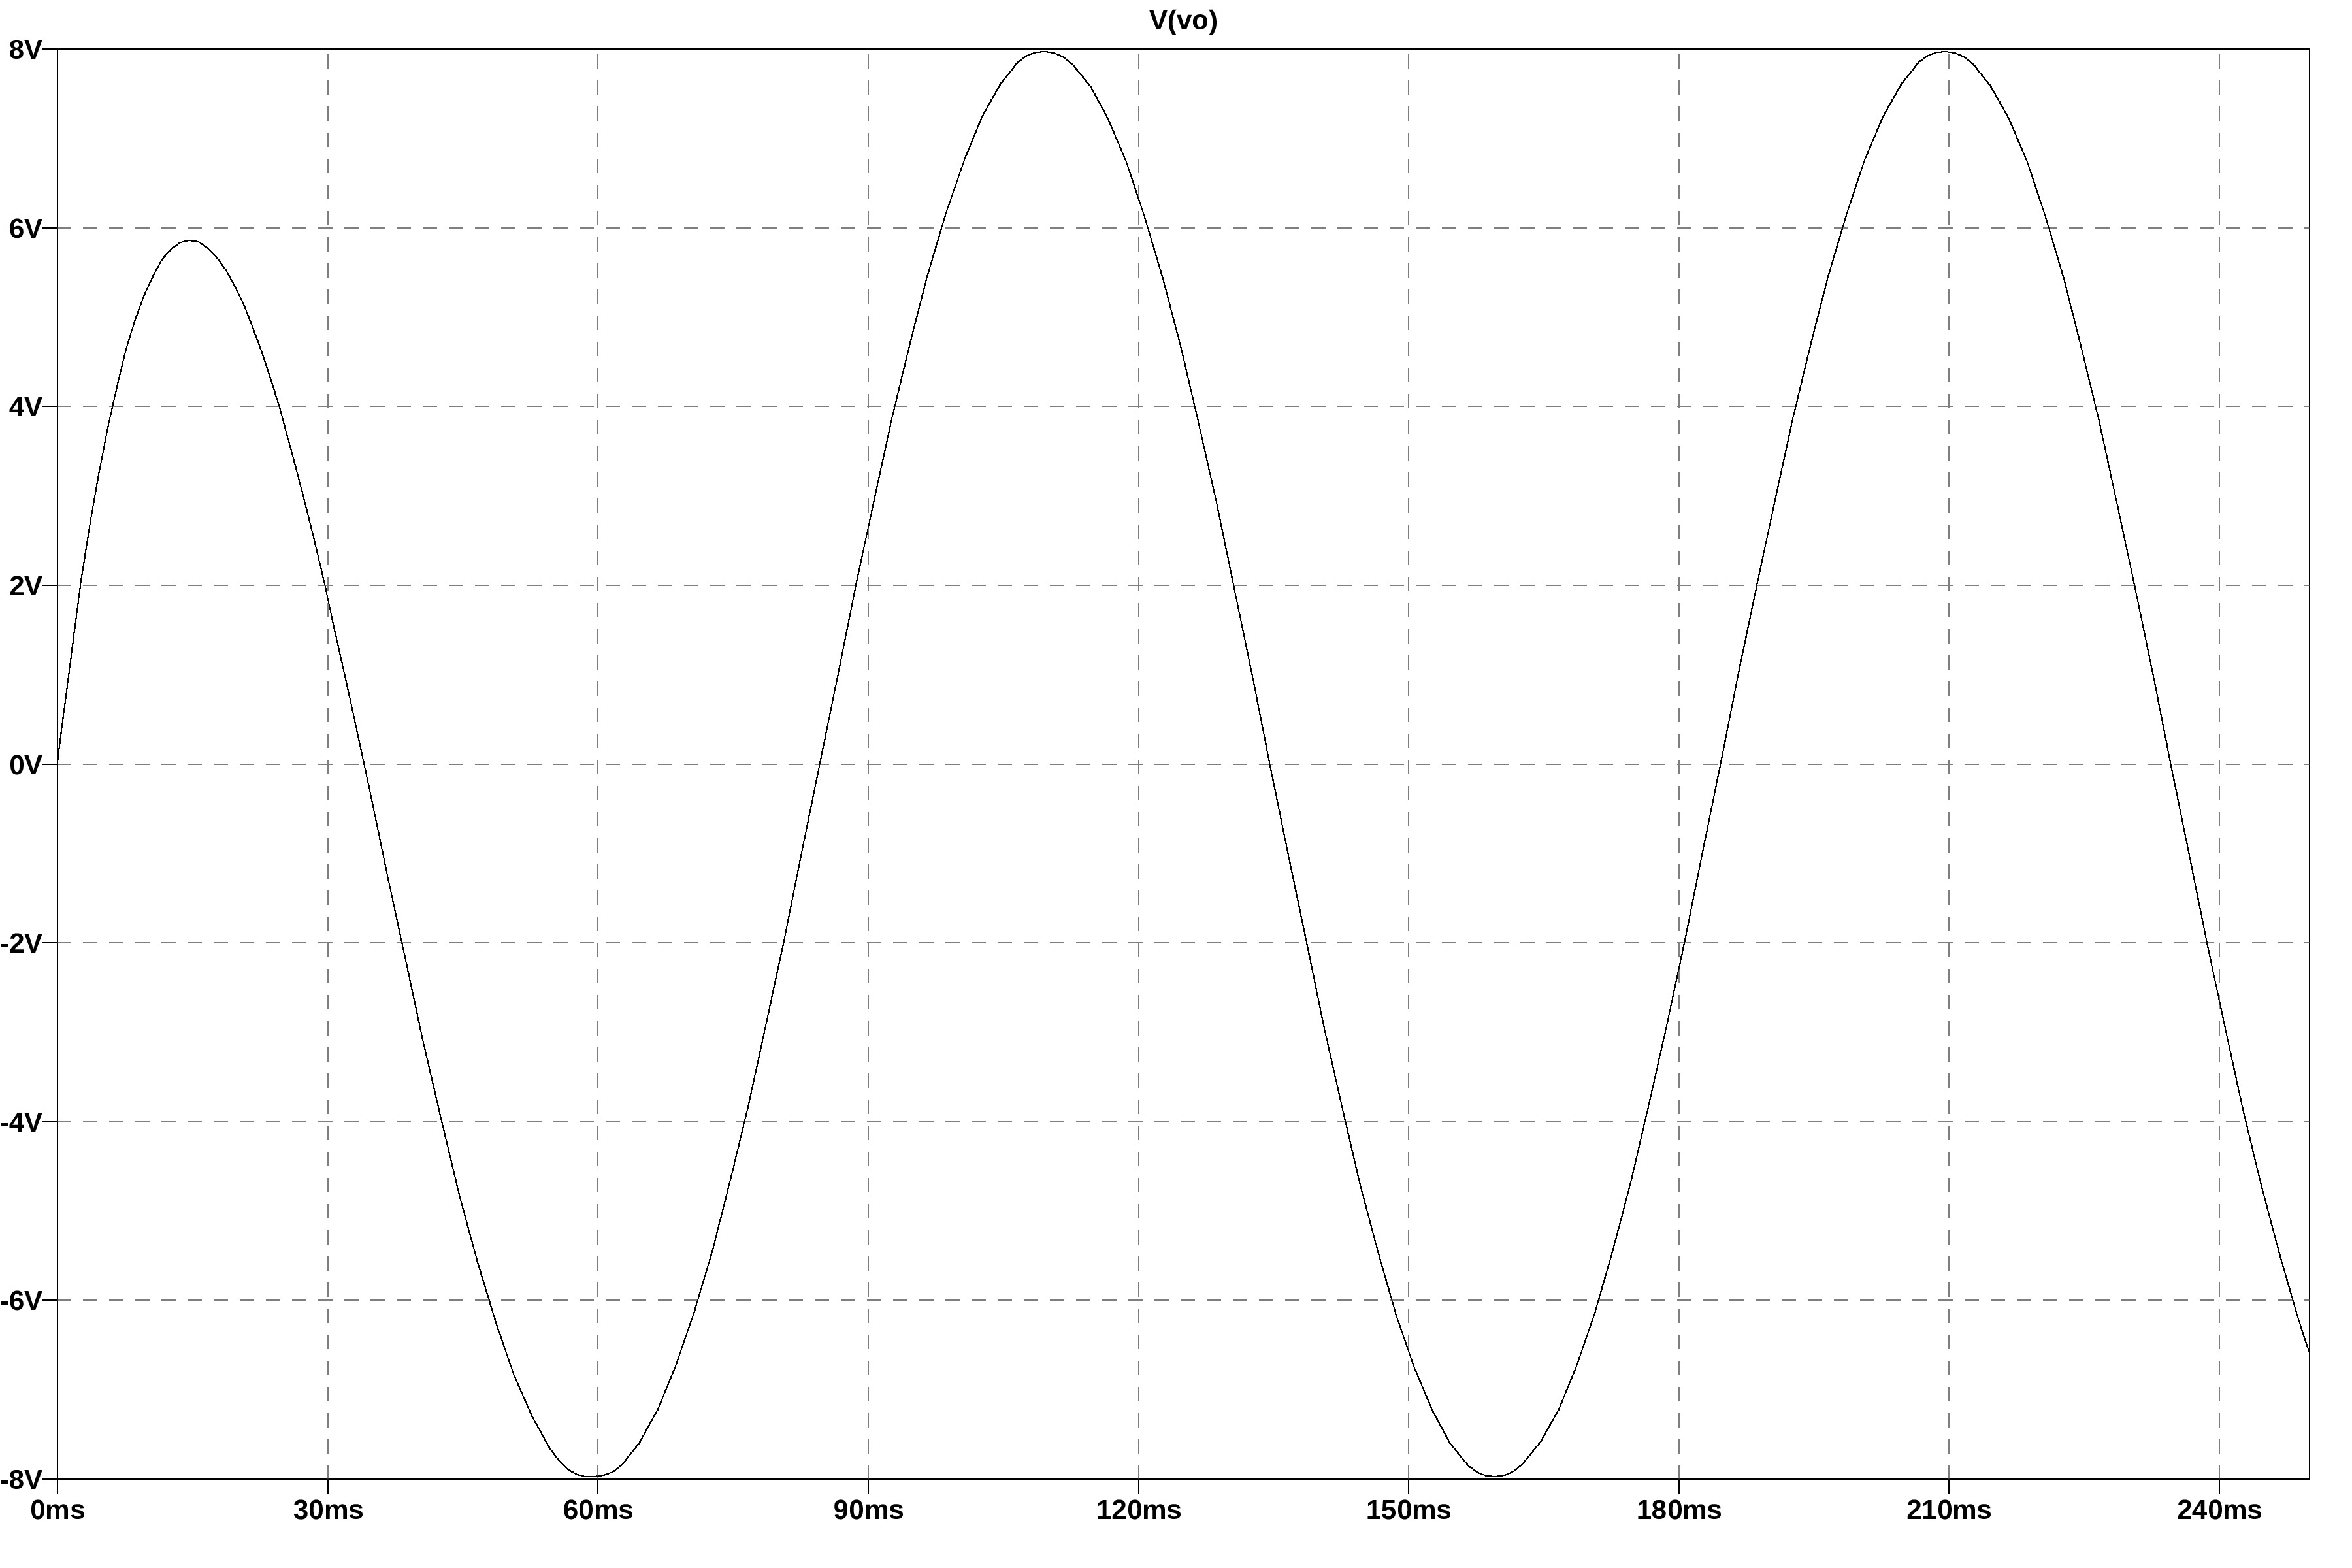
\includegraphics[width=14cm]{graph/1d5.jpg}
  \caption{Audio Amplifier - Output voltage with an amplitude of the imput voltage equal to $1.28091V$, frequency equal to $10Hz$, $R_2$ equal to $109775.2\Omega$}
  \label{1d5graph}
\end{figure}

\subsection{Output voltage waveform - $R_2 = 109775.2\Omega$ - $V_{in} = 2 \cdot |V_{in MAX} |$}
The netlist used for plot the output voltage waveform with a double input voltage relatively to the maximum input voltage calculated is:\\
\lstinputlisting{netlist/1d5b.cir}

\begin{figure}[H]
  \centering
  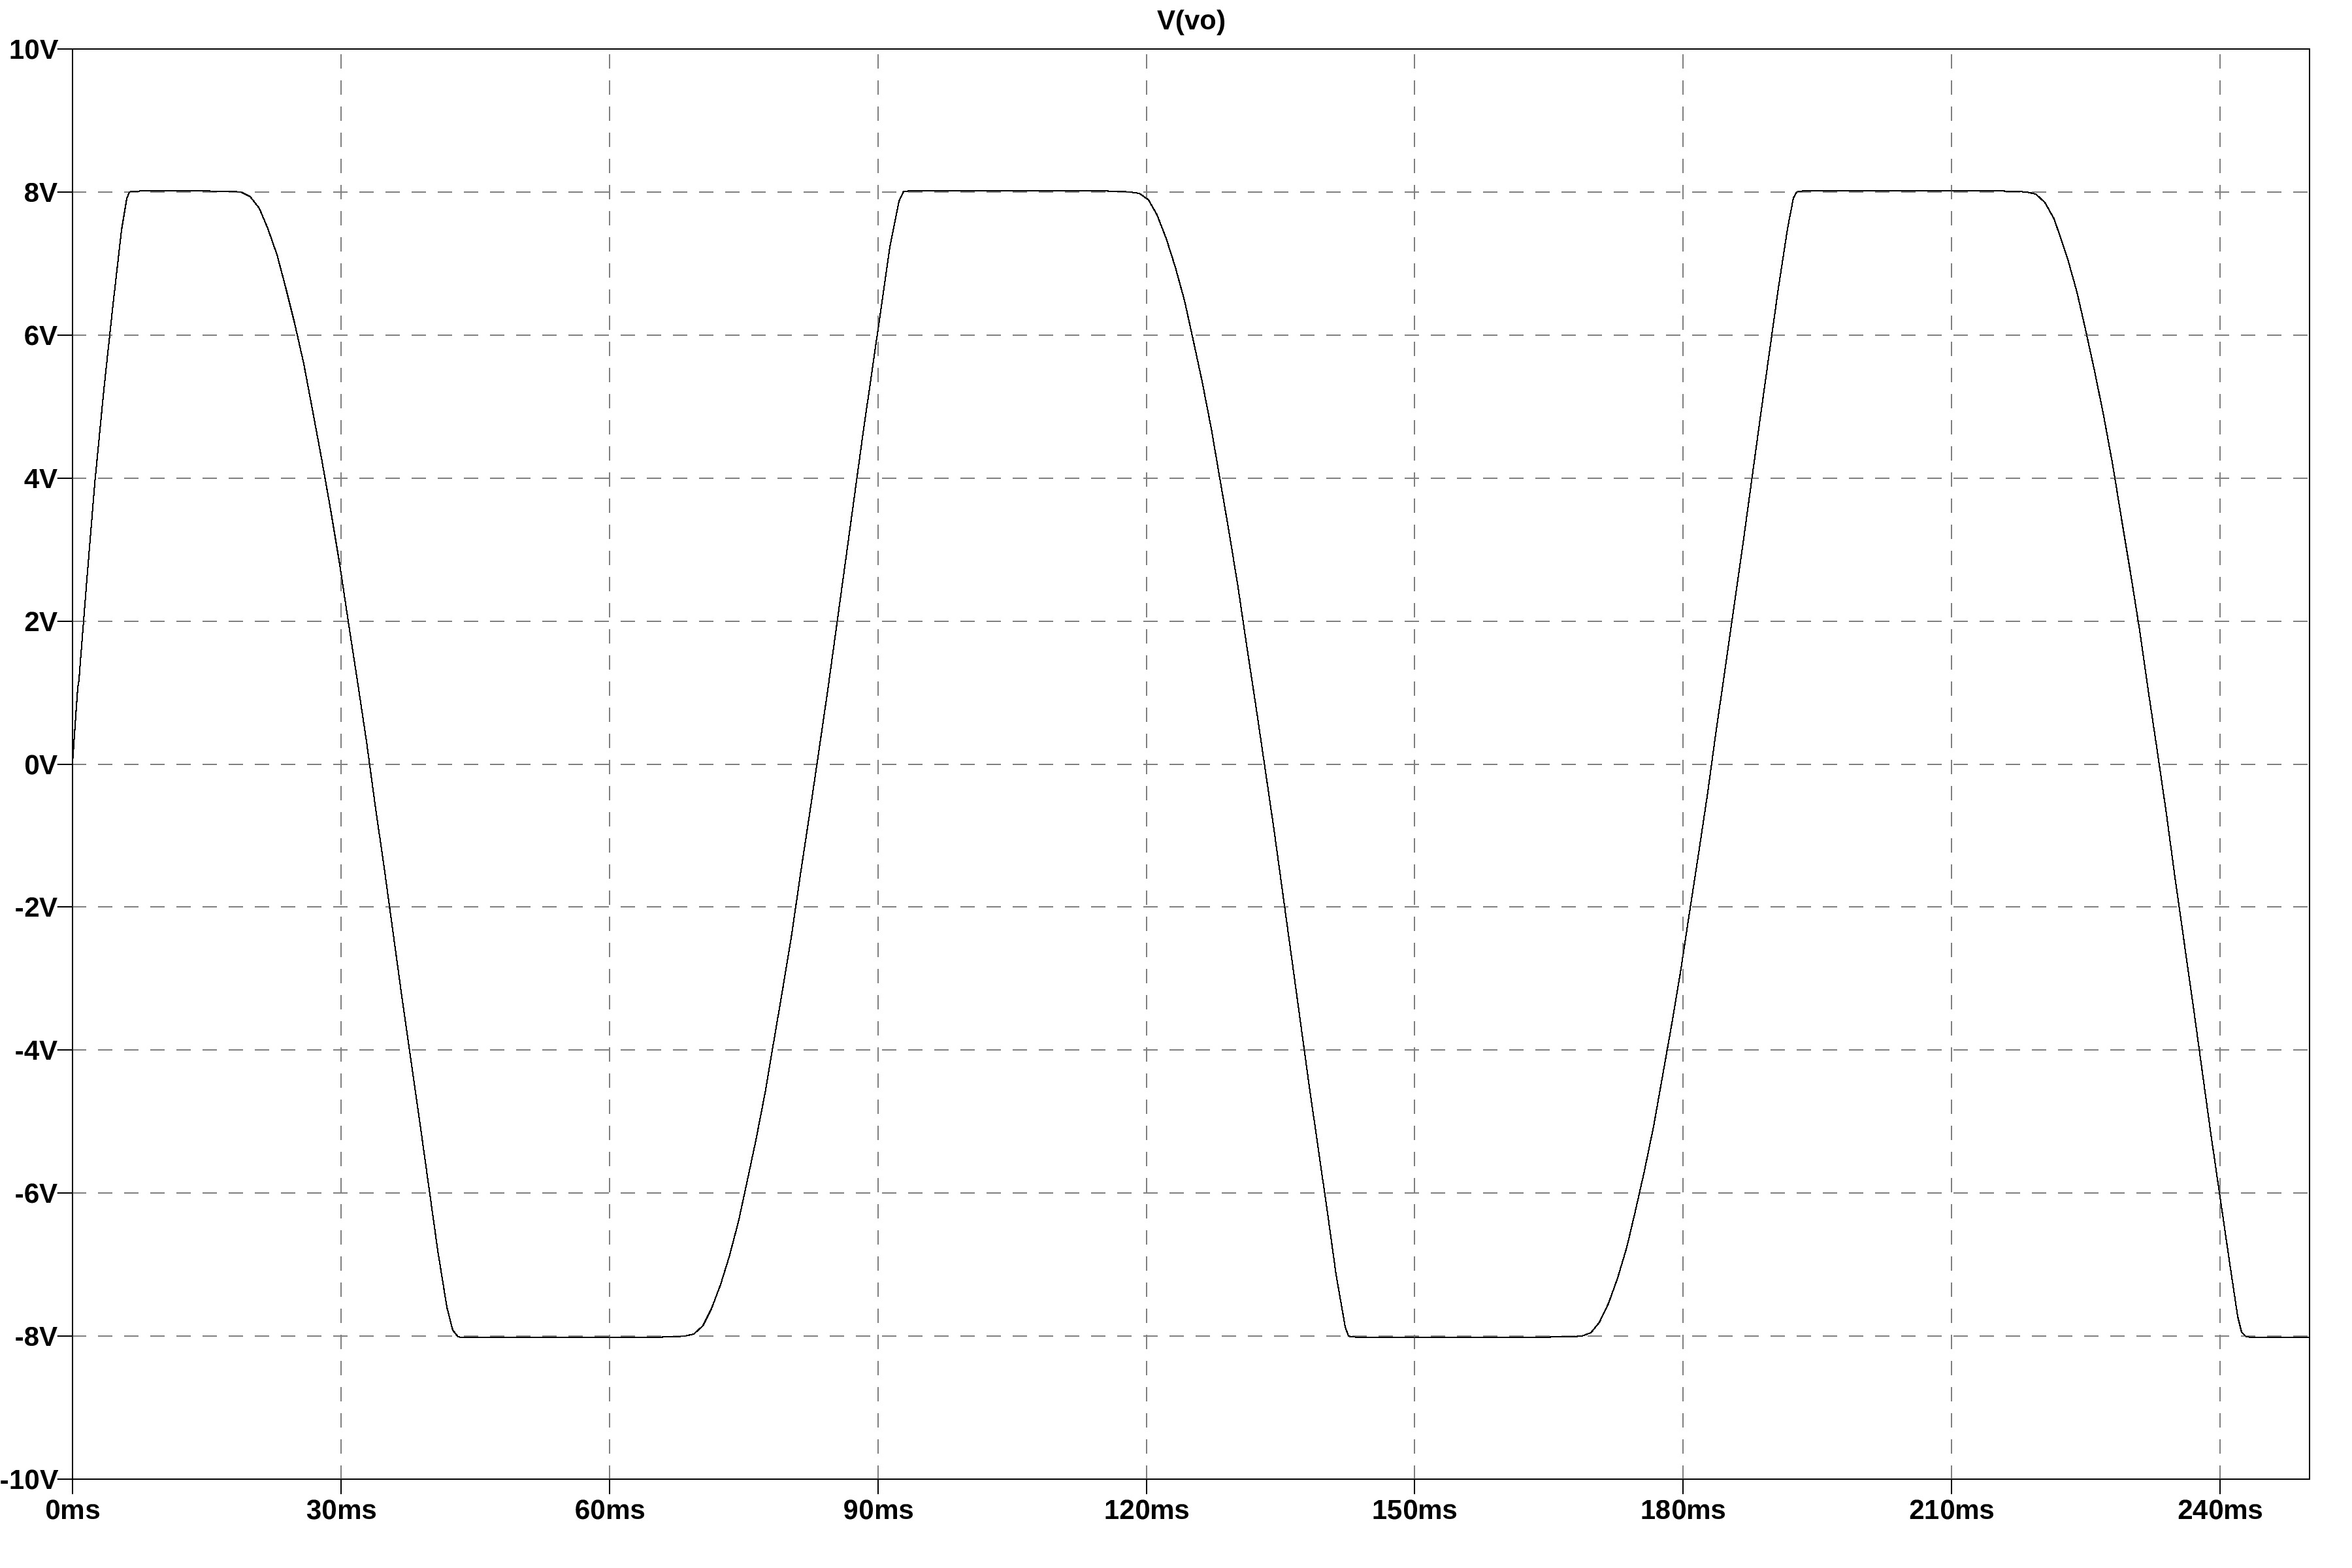
\includegraphics[width=14cm]{graph/1d5b.jpg}
  \caption{Audio Amplifier - Output voltage with an amplitude of the imput voltage equal to $2 \cdot 1.28091V$, frequency equal to $10Hz$, $R_2$ equal to $109775.2\Omega$}
  \label{1d5bgraph}
\end{figure}

The graph generated is presented on the figure \ref{1d5bgraph}.\\

\section{Power delivered to the amplifier}

\begin{equation}
  P_{DC} = V_{dd} \cdot I_{dd} + V_{ss} \cdot I_{ss}
\end{equation}

\subsection{Case A - $R_2 = 100k\Omega$ $V_{in} = 2 \cdot 1.36701V$}
\lstinputlisting{netlist/1d6.cir}

$$P_{DC} = 10V \cdot (-0.00736621A) + (-10V) \cdot (+0.00736621 A) = -0.14732420W$$

\subsection{Case B - $R_2 = 109775.2\Omega$ $V_{in} = 2 \cdot 1.28091V$}
\lstinputlisting{netlist/1d6b.cir}

$$P_{DC} = 10V \cdot (-0.00736621A) + (-10V) \cdot (+0.00736621 A) = -0.14732420W$$

\chapter{Band Pass Amplifier}

\begin{figure}[H]
  \centering
  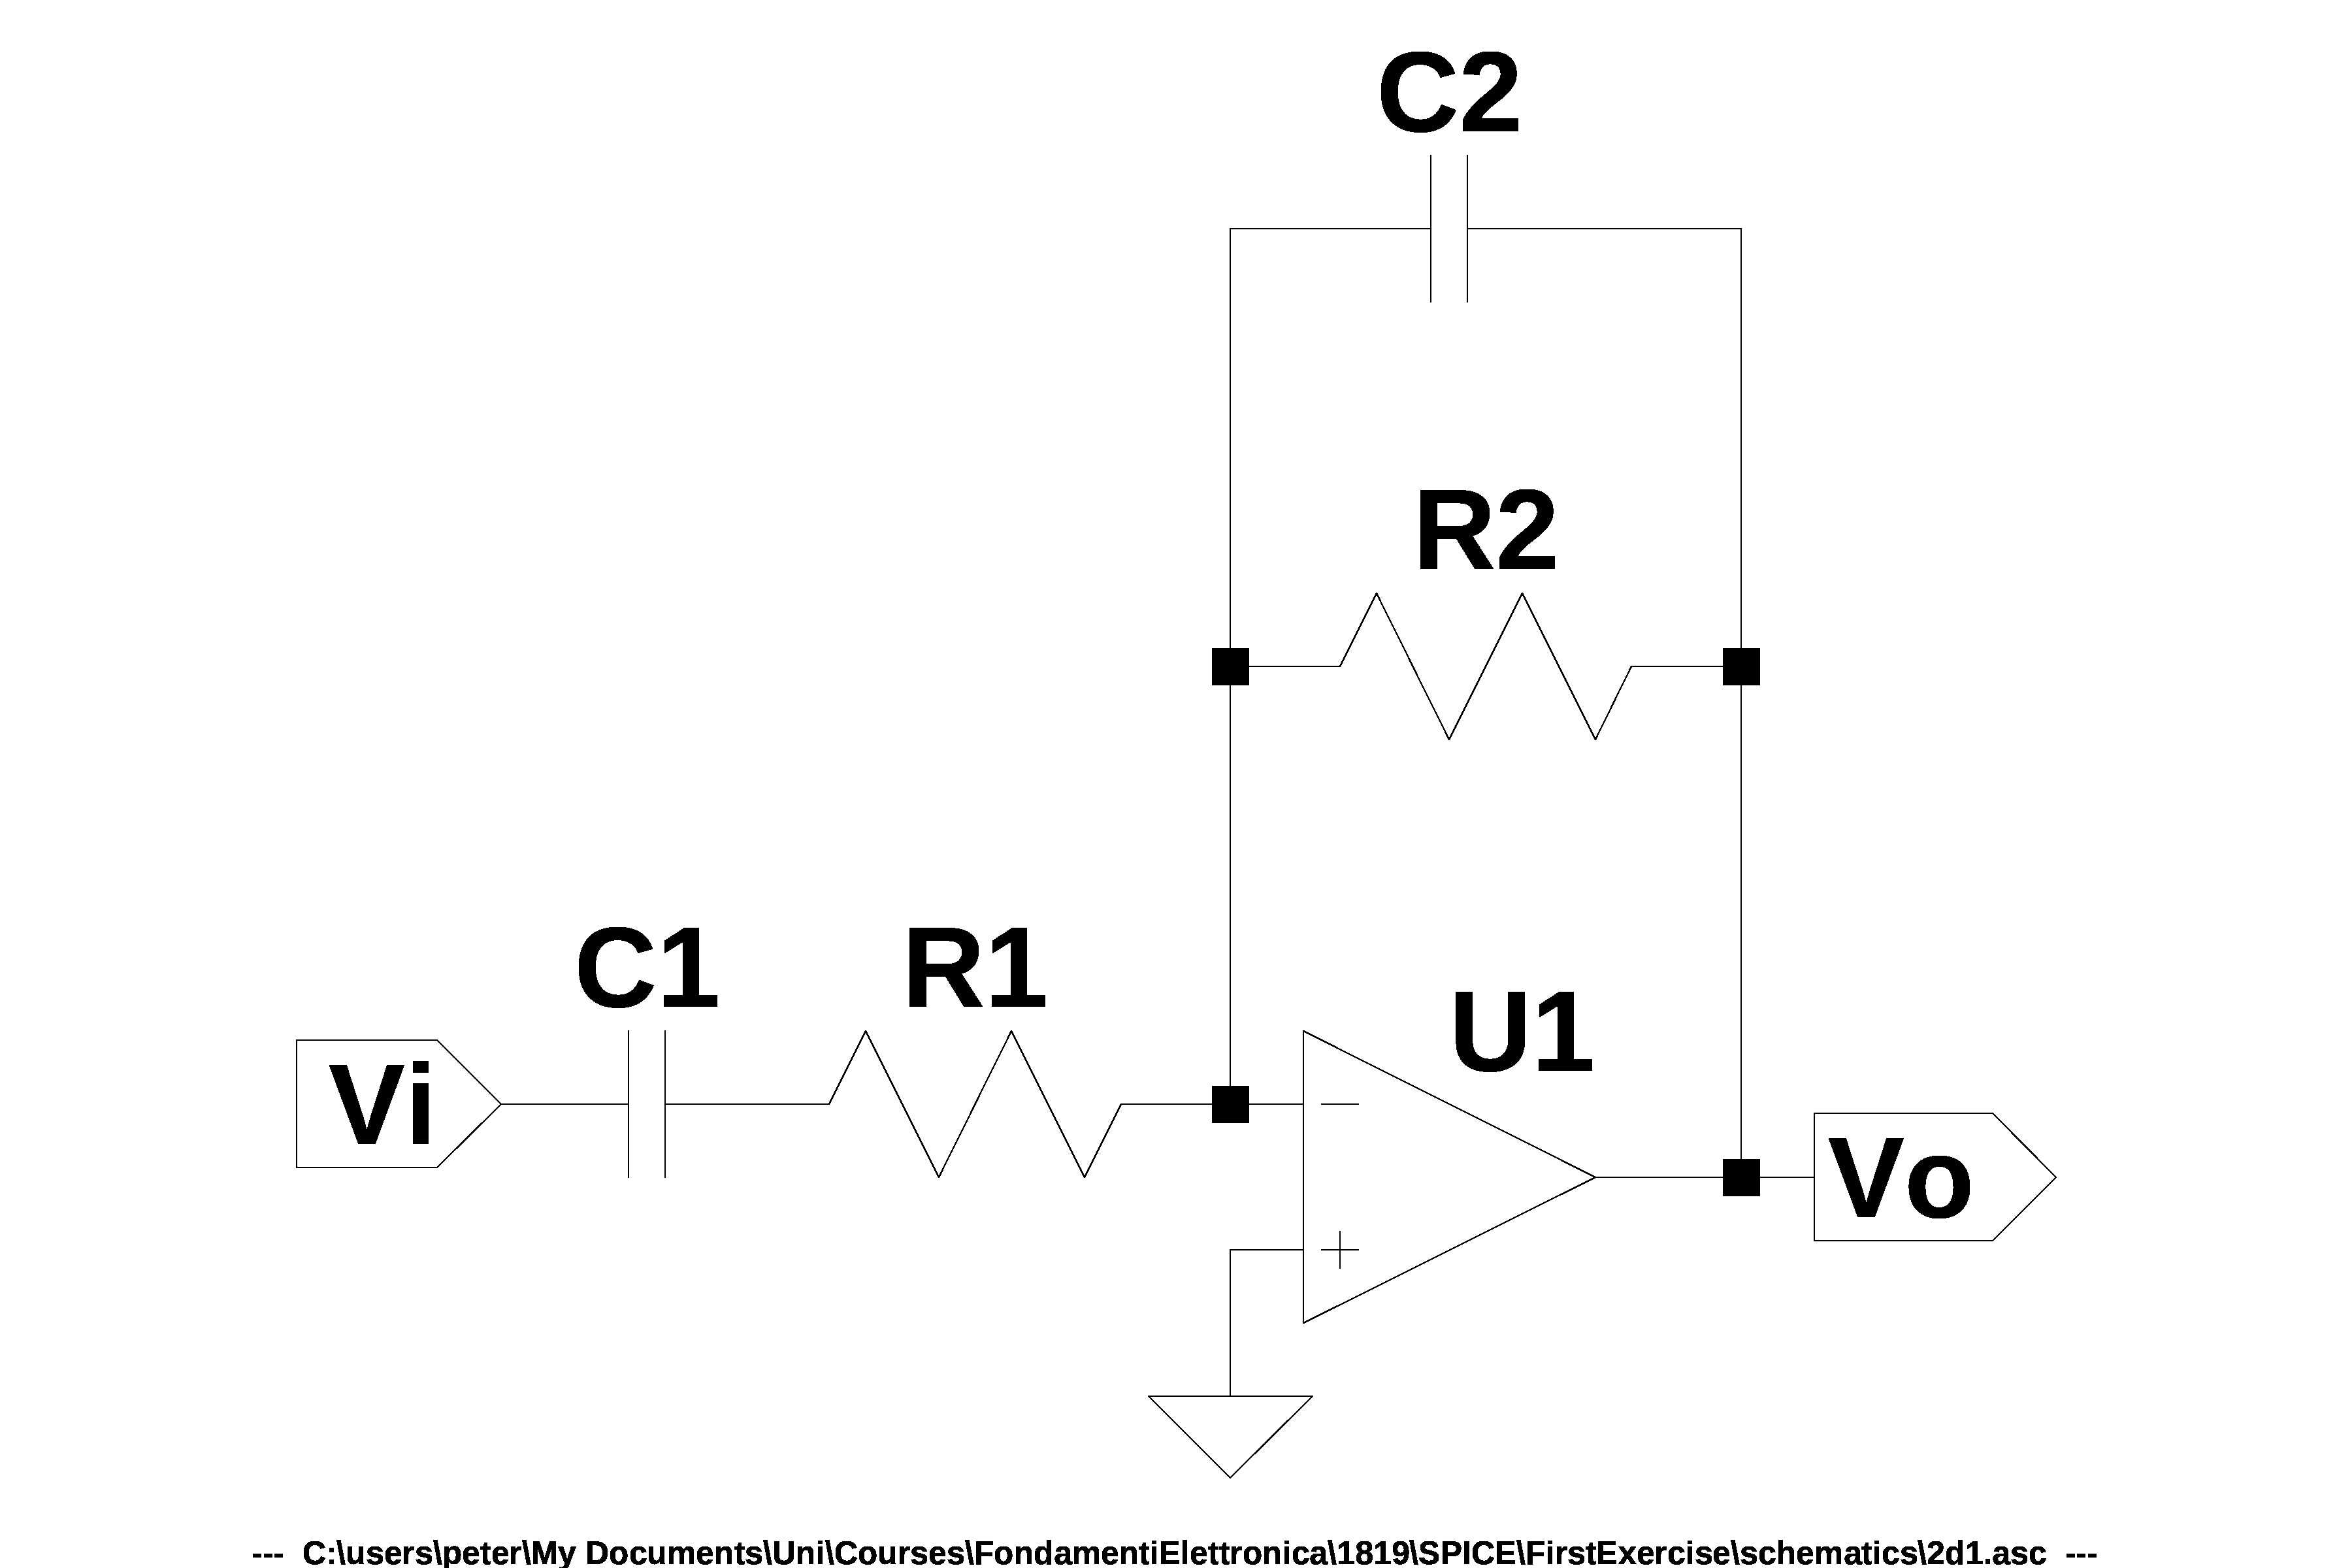
\includegraphics[width=10cm]{schematics/2d1.jpg}
  \caption{Band pass amplifier - Circuit schematics}
  \label{2d1schematics}
\end{figure}

\section{Transfer function}

\begin{align}
  V_o(s) = - (C_2 \parallel R_2) \cdot \frac{V_i(s)}{\frac{1}{sC_1}+R_1} \nonumber \\
  V_o(s) = - \frac{\frac{1}{sC_2} \cdot R_2}{\frac{1}{sC_2}+R_2} \cdot \frac{sC_2}{sC_2} \cdot \frac{V_i(s)}{\frac{1}{sC_1}+R_1} \cdot \frac{sC_1}{sC_1} \nonumber \\
  V_o(s) = - \frac{R_2}{1+sC_2R_2} \cdot \frac{V_i(s) \cdot sC_1}{1+sC_1R_1} \nonumber \\
  \frac{V_o(s)}{V_i(s)} = - \frac{sC_1R_2}{(1+sC_1R_1)(1+sC_2R_2)}
\end{align}

\section{Determining capacitances and resistances}
The conditions to respect are described by the system \ref{eq:conditions}.
\begin{equation}
  \left\{
  \begin{array}{l}
    R_1 = 1097752\Omega/1000 \\
    \omega_1 = \frac{1}{C_1R_2} = 10 \\
    \omega_2 = \frac{1}{C_1R_1} = 10^3 \\
    \omega_3 = \frac{1}{C_2R_2} = 10^6
  \end{array}
  \right. \label{eq:conditions}
\end{equation}

Resolving the system it's possible to find the value of the circuit's capacitances and resistances (system \ref{eq:cap_n_res}).
\begin{equation}
  \left\{
  \begin{array}{l}
    R_1 = 1097.752\Omega\\
    R_2 = 109775.2\Omega\\
    C_1 = 910.95256nF\\
    C_2 = 9.10953pF\\
  \end{array}
  \right. \label{eq:cap_n_res}
\end{equation}

\section{Bode plot}
\subsection{Netlist}
\lstinputlisting{netlist/2d3.cir}

\subsection{Graph}
\begin{figure}[H]
  \centering
  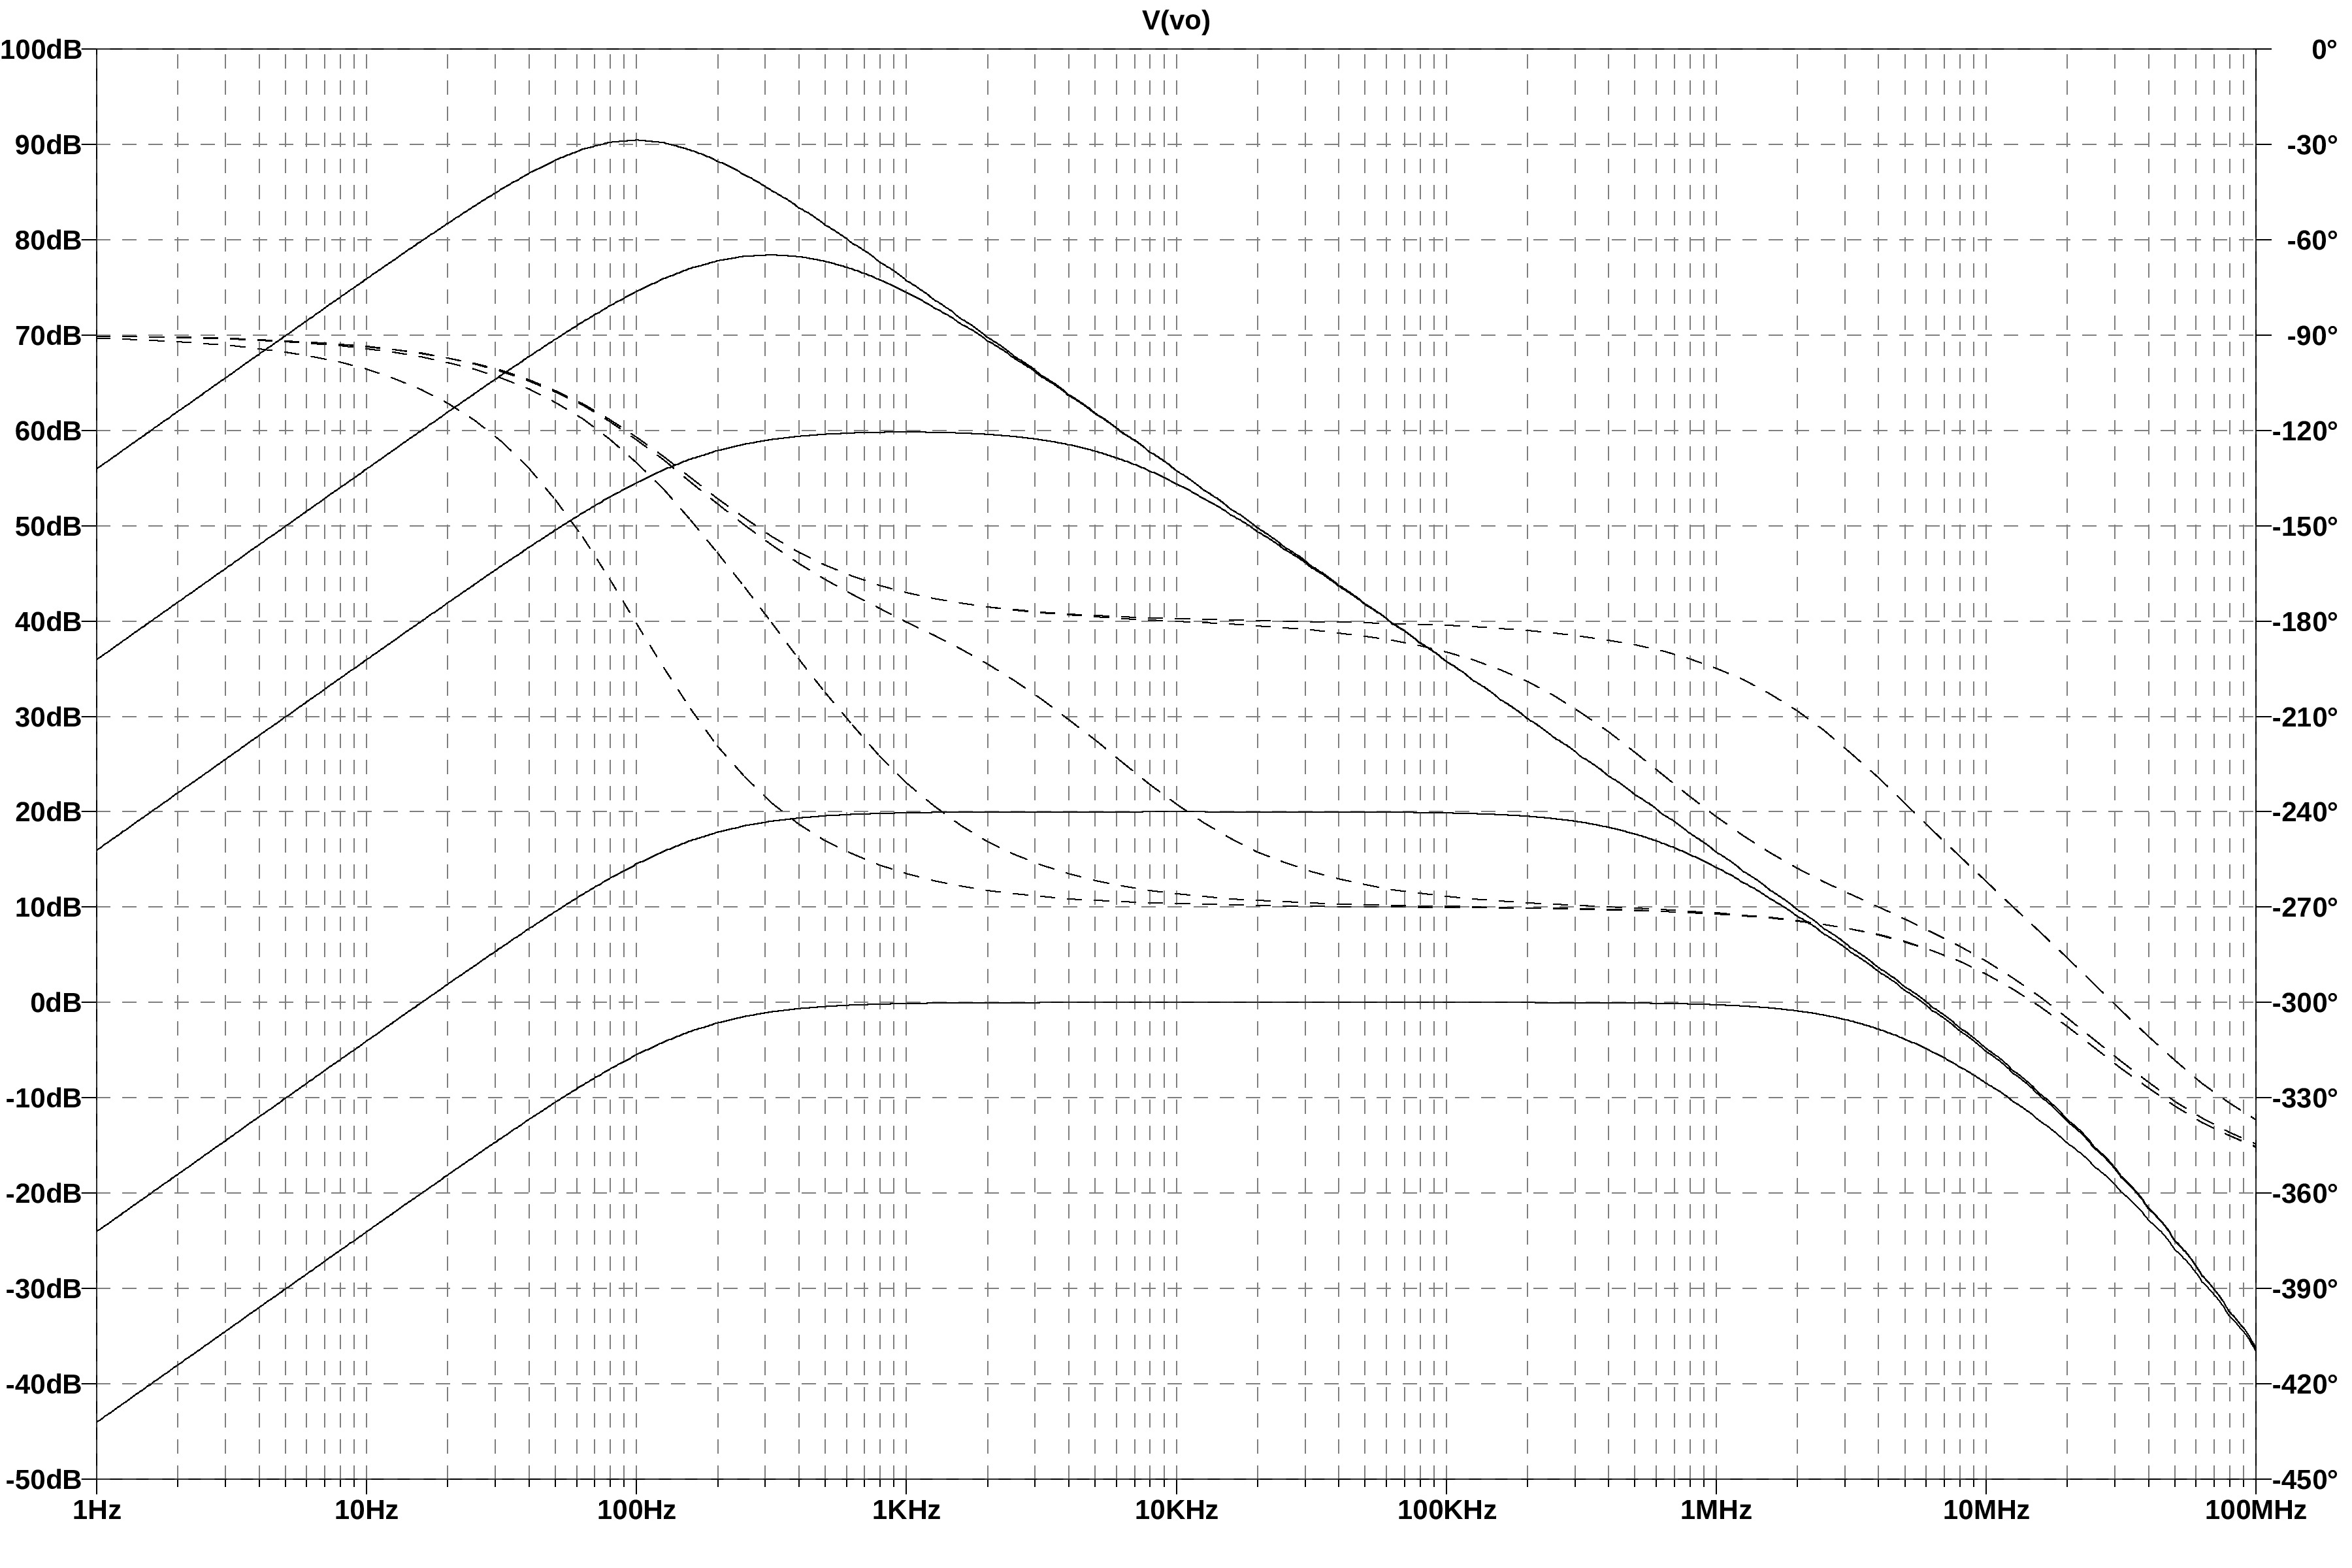
\includegraphics[width=14cm]{graph/2d3.jpg}
  \caption{Band pass amplifier - Bode plot}
  \label{2d3graph}
\end{figure}

\section{Output voltage}
\subsection{$Vin$ frequency $10Hz$ $100Hz$}
\lstinputlisting{netlist/2d4a.cir}

\begin{figure}[H]
  \centering
  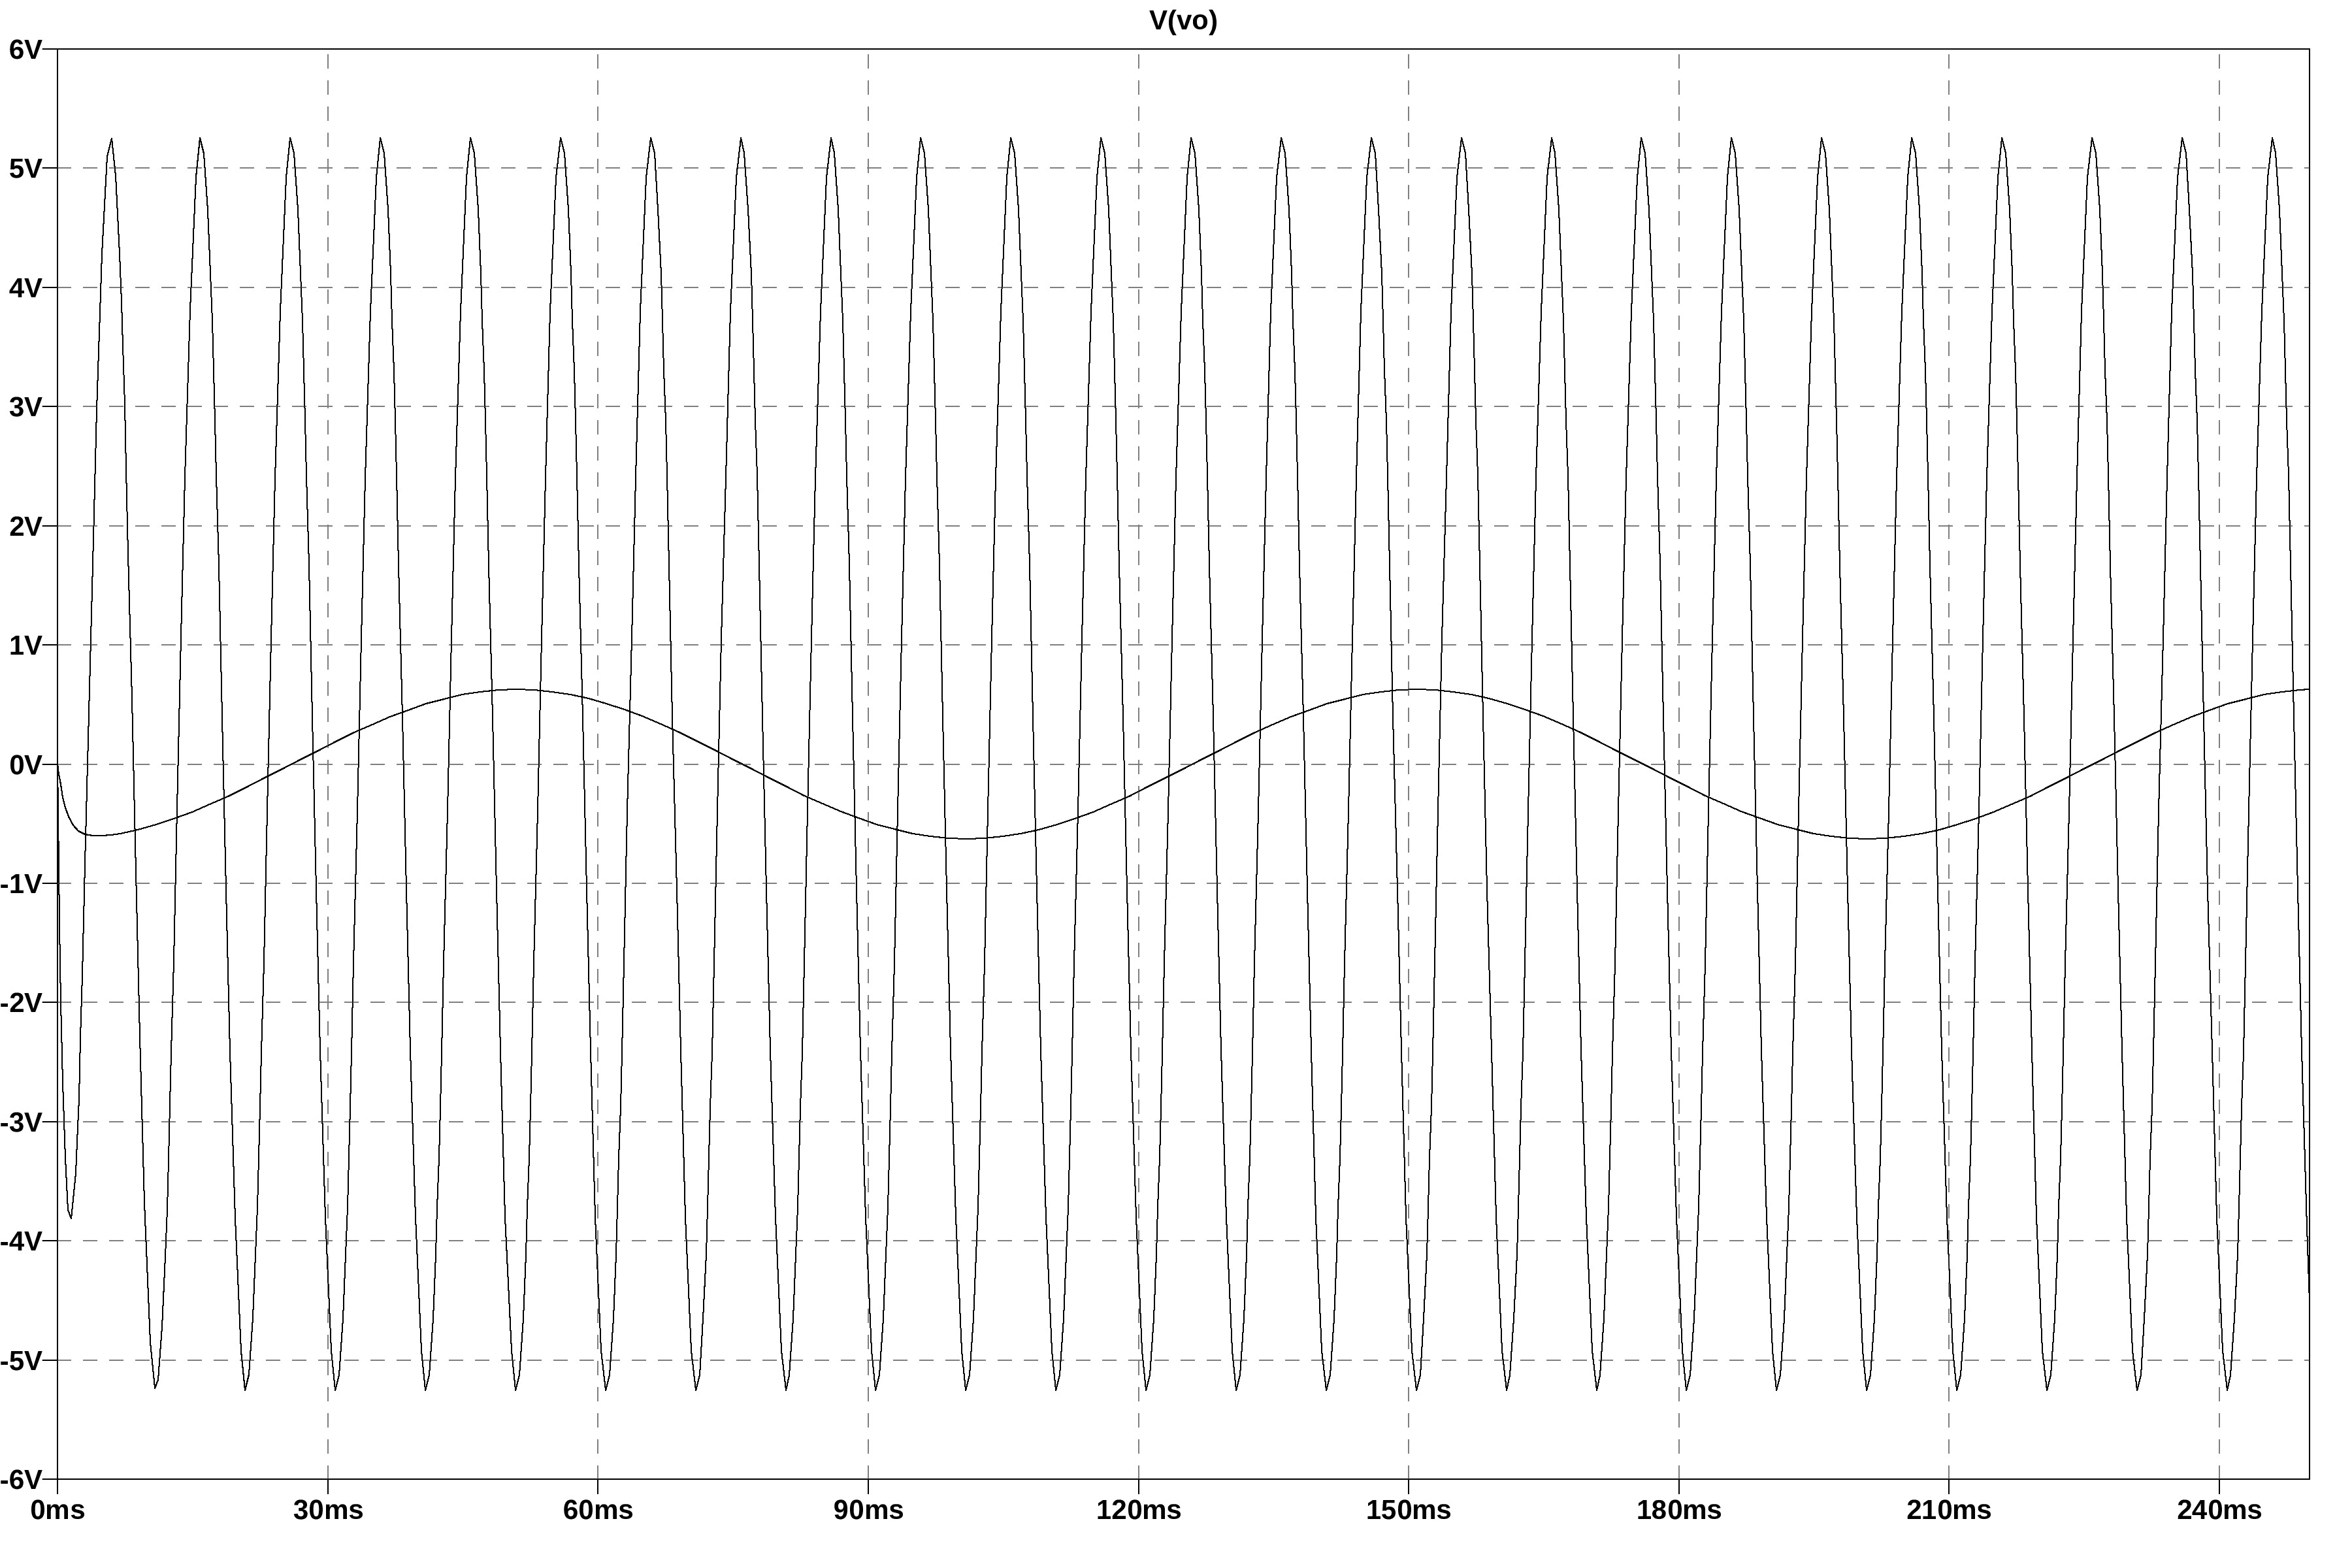
\includegraphics[width=14cm]{graph/2d4a.jpg}
  \caption{Band pass amplifier - Bode plot - $Vin$ frequency $10Hz$ $100Hz$}
  \label{2d4agraph}
\end{figure}

\subsection{$Vin$ frequency $1kHz$ $10kHz$ $100kHz$}
\lstinputlisting{netlist/2d4b.cir}

\begin{figure}[H]
  \centering
  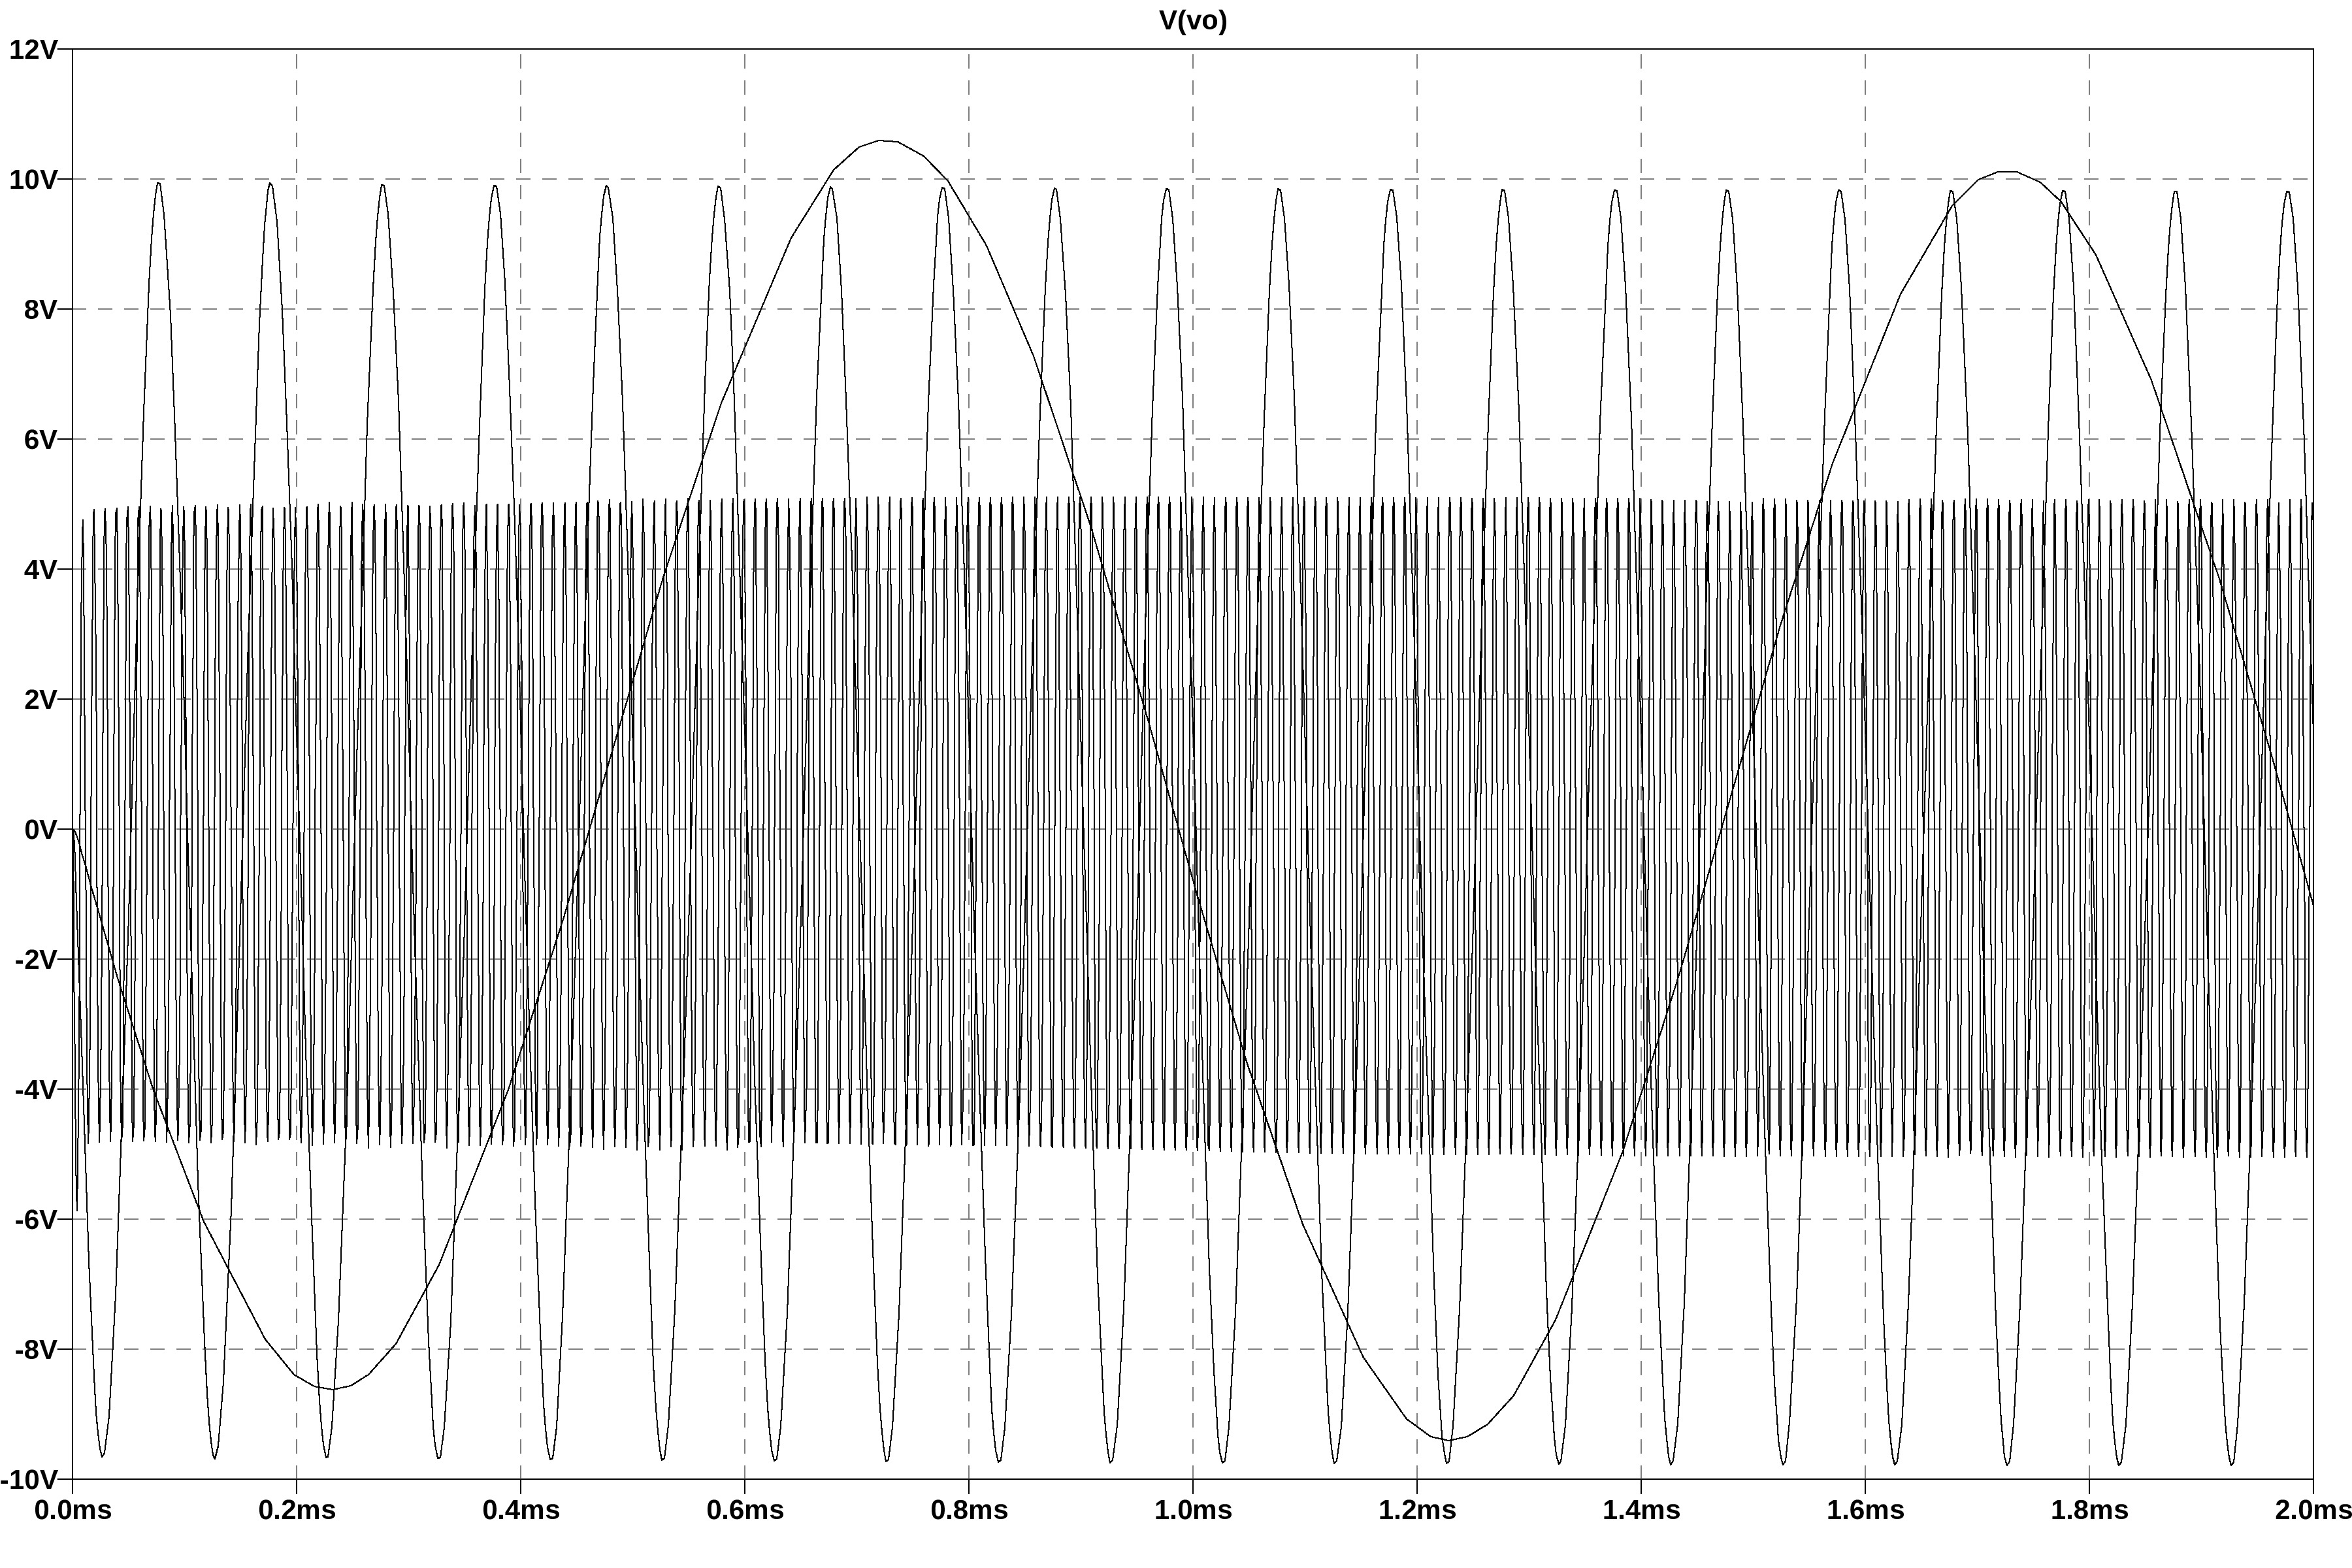
\includegraphics[width=14cm]{graph/2d4b.jpg}
  \caption{Band pass amplifier - Bode plot - $Vin$ frequency $1kHz$ $10kHz$ $100kHz$}
  \label{2d4bgraph}
\end{figure}

\subsection{$Vin$ frequency $1MEGHz$ $10MEGHz$ $100MEGHz$}
\lstinputlisting{netlist/2d4c.cir}

\begin{figure}[H]
  \centering
  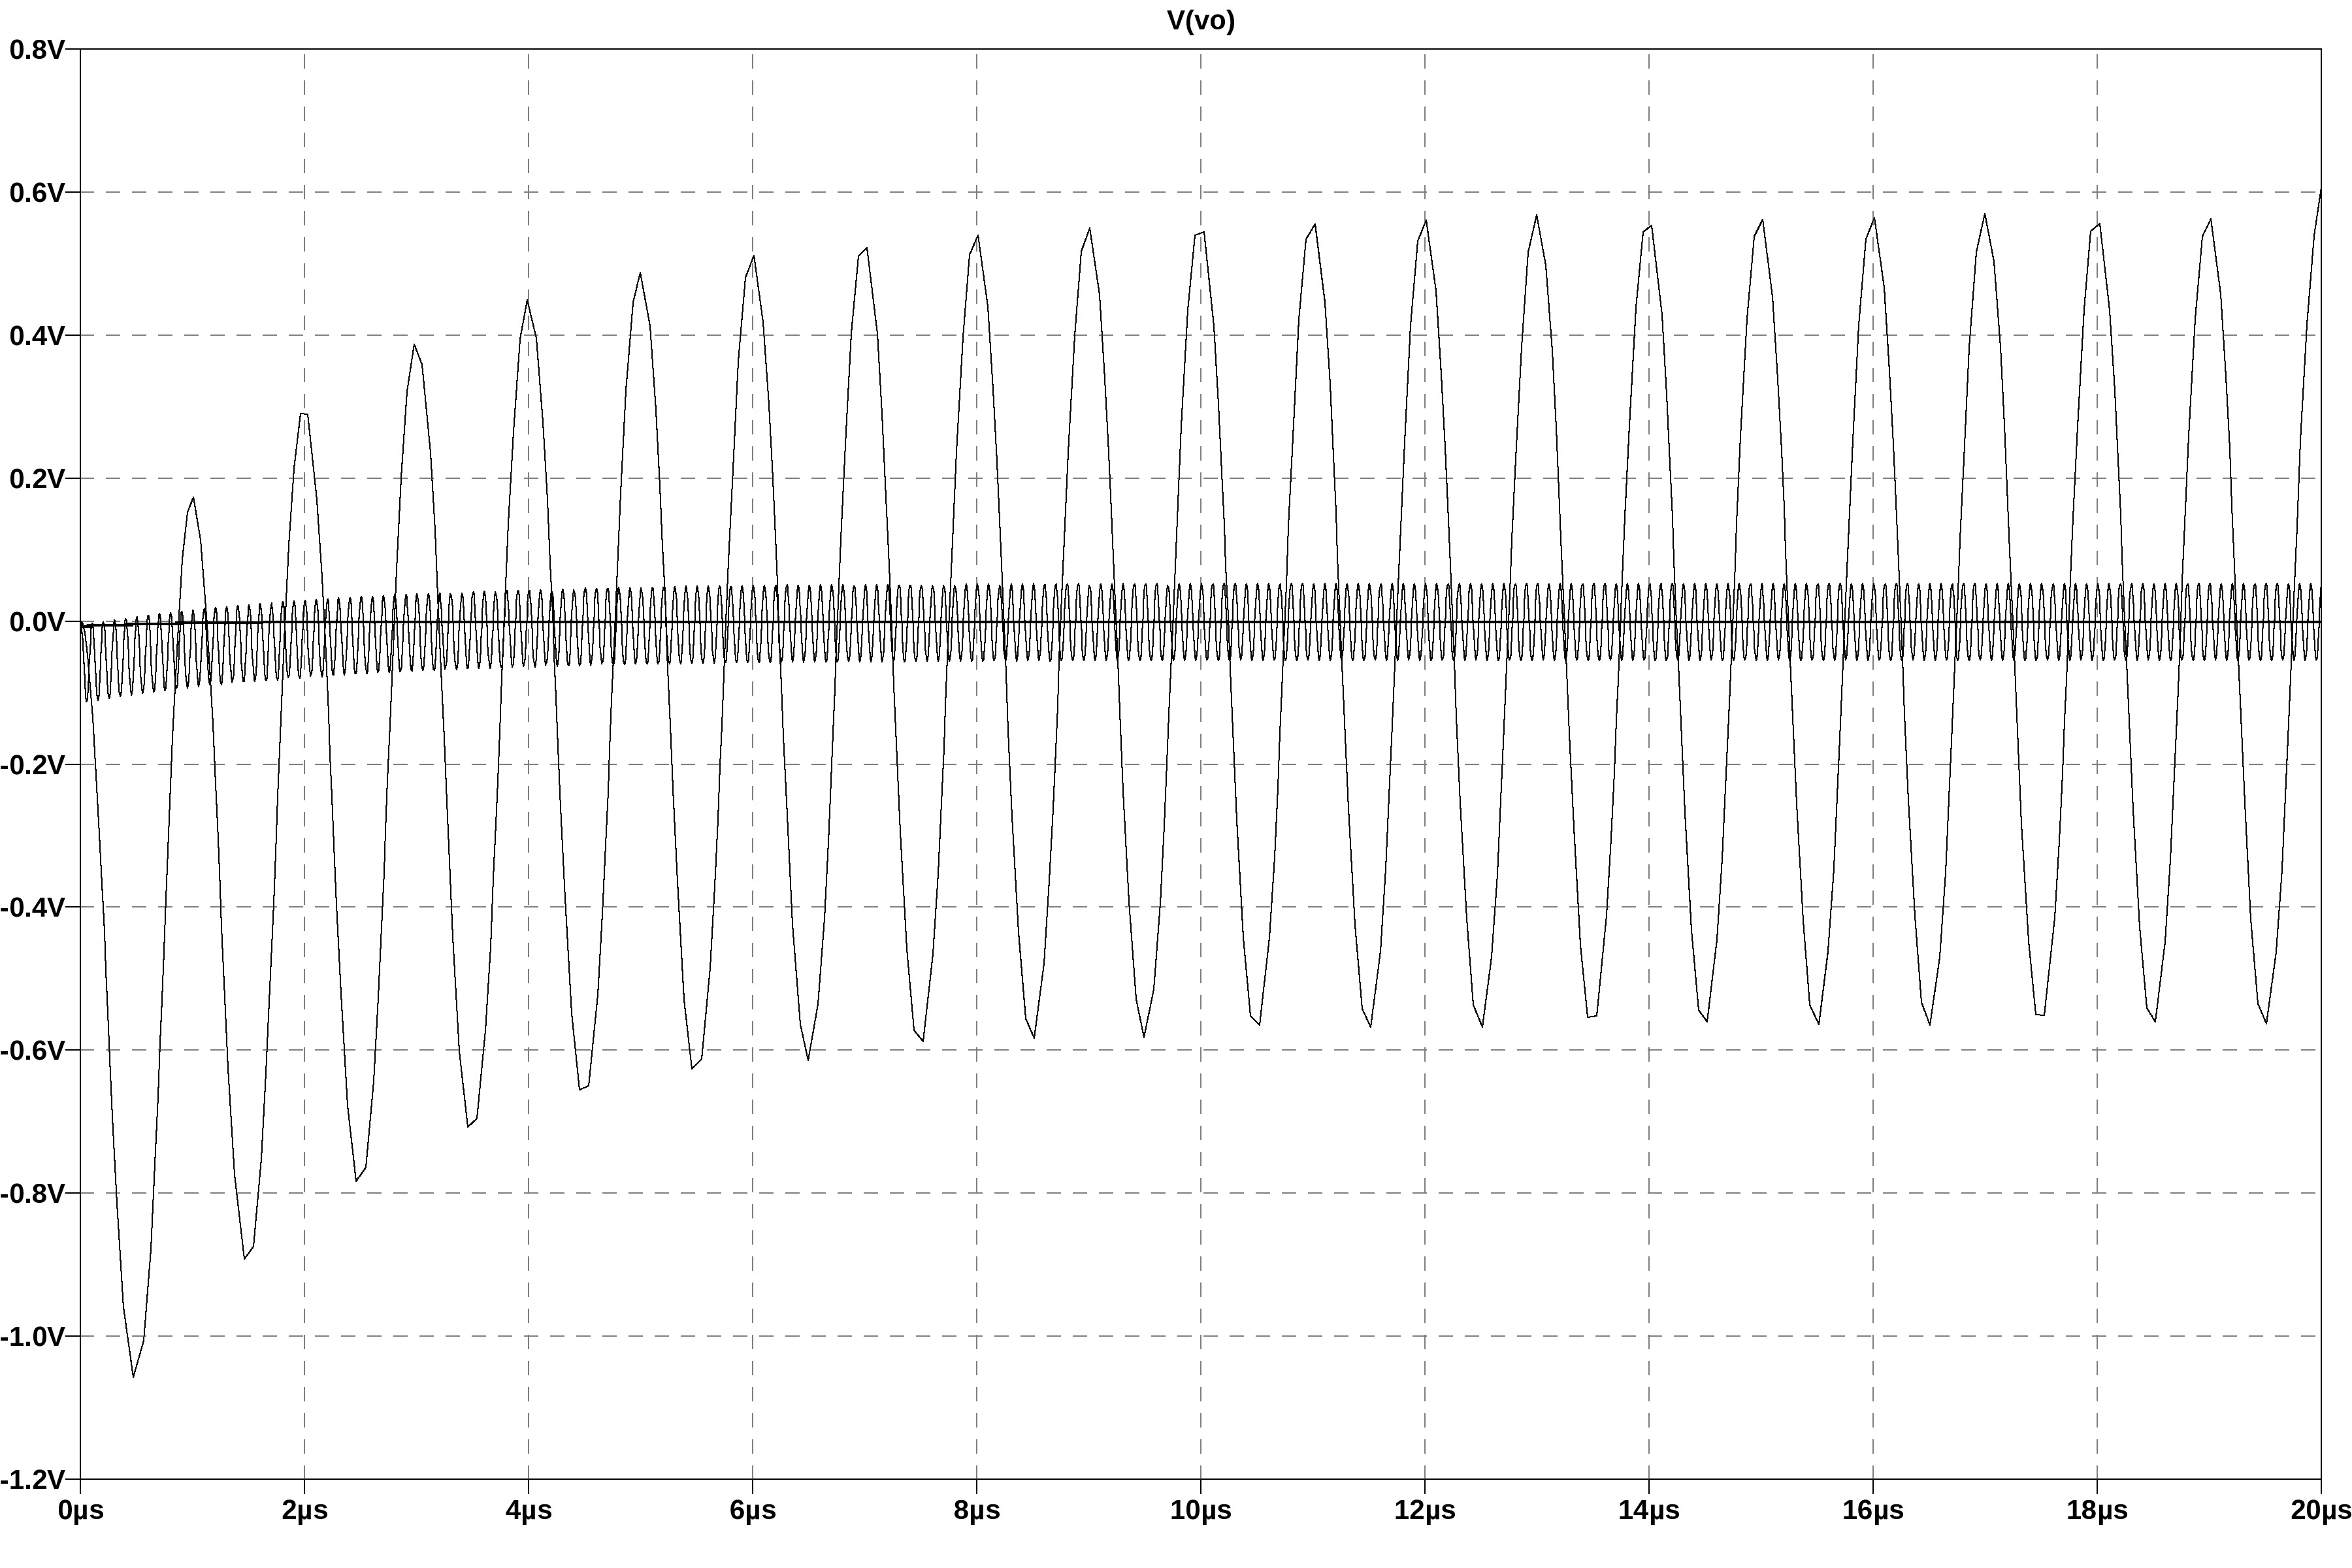
\includegraphics[width=14cm]{graph/2d4c.jpg}
  \caption{Band pass amplifier - Bode plot - $Vin$ frequency $1MEGHz$ $10MEGHz$ $100MEGHz$}
  \label{2d4cgraph}
\end{figure}

\chapter{Front-end amplifier for resistive bridge with resistometric sensor}

\begin{figure}[H]
  \centering
  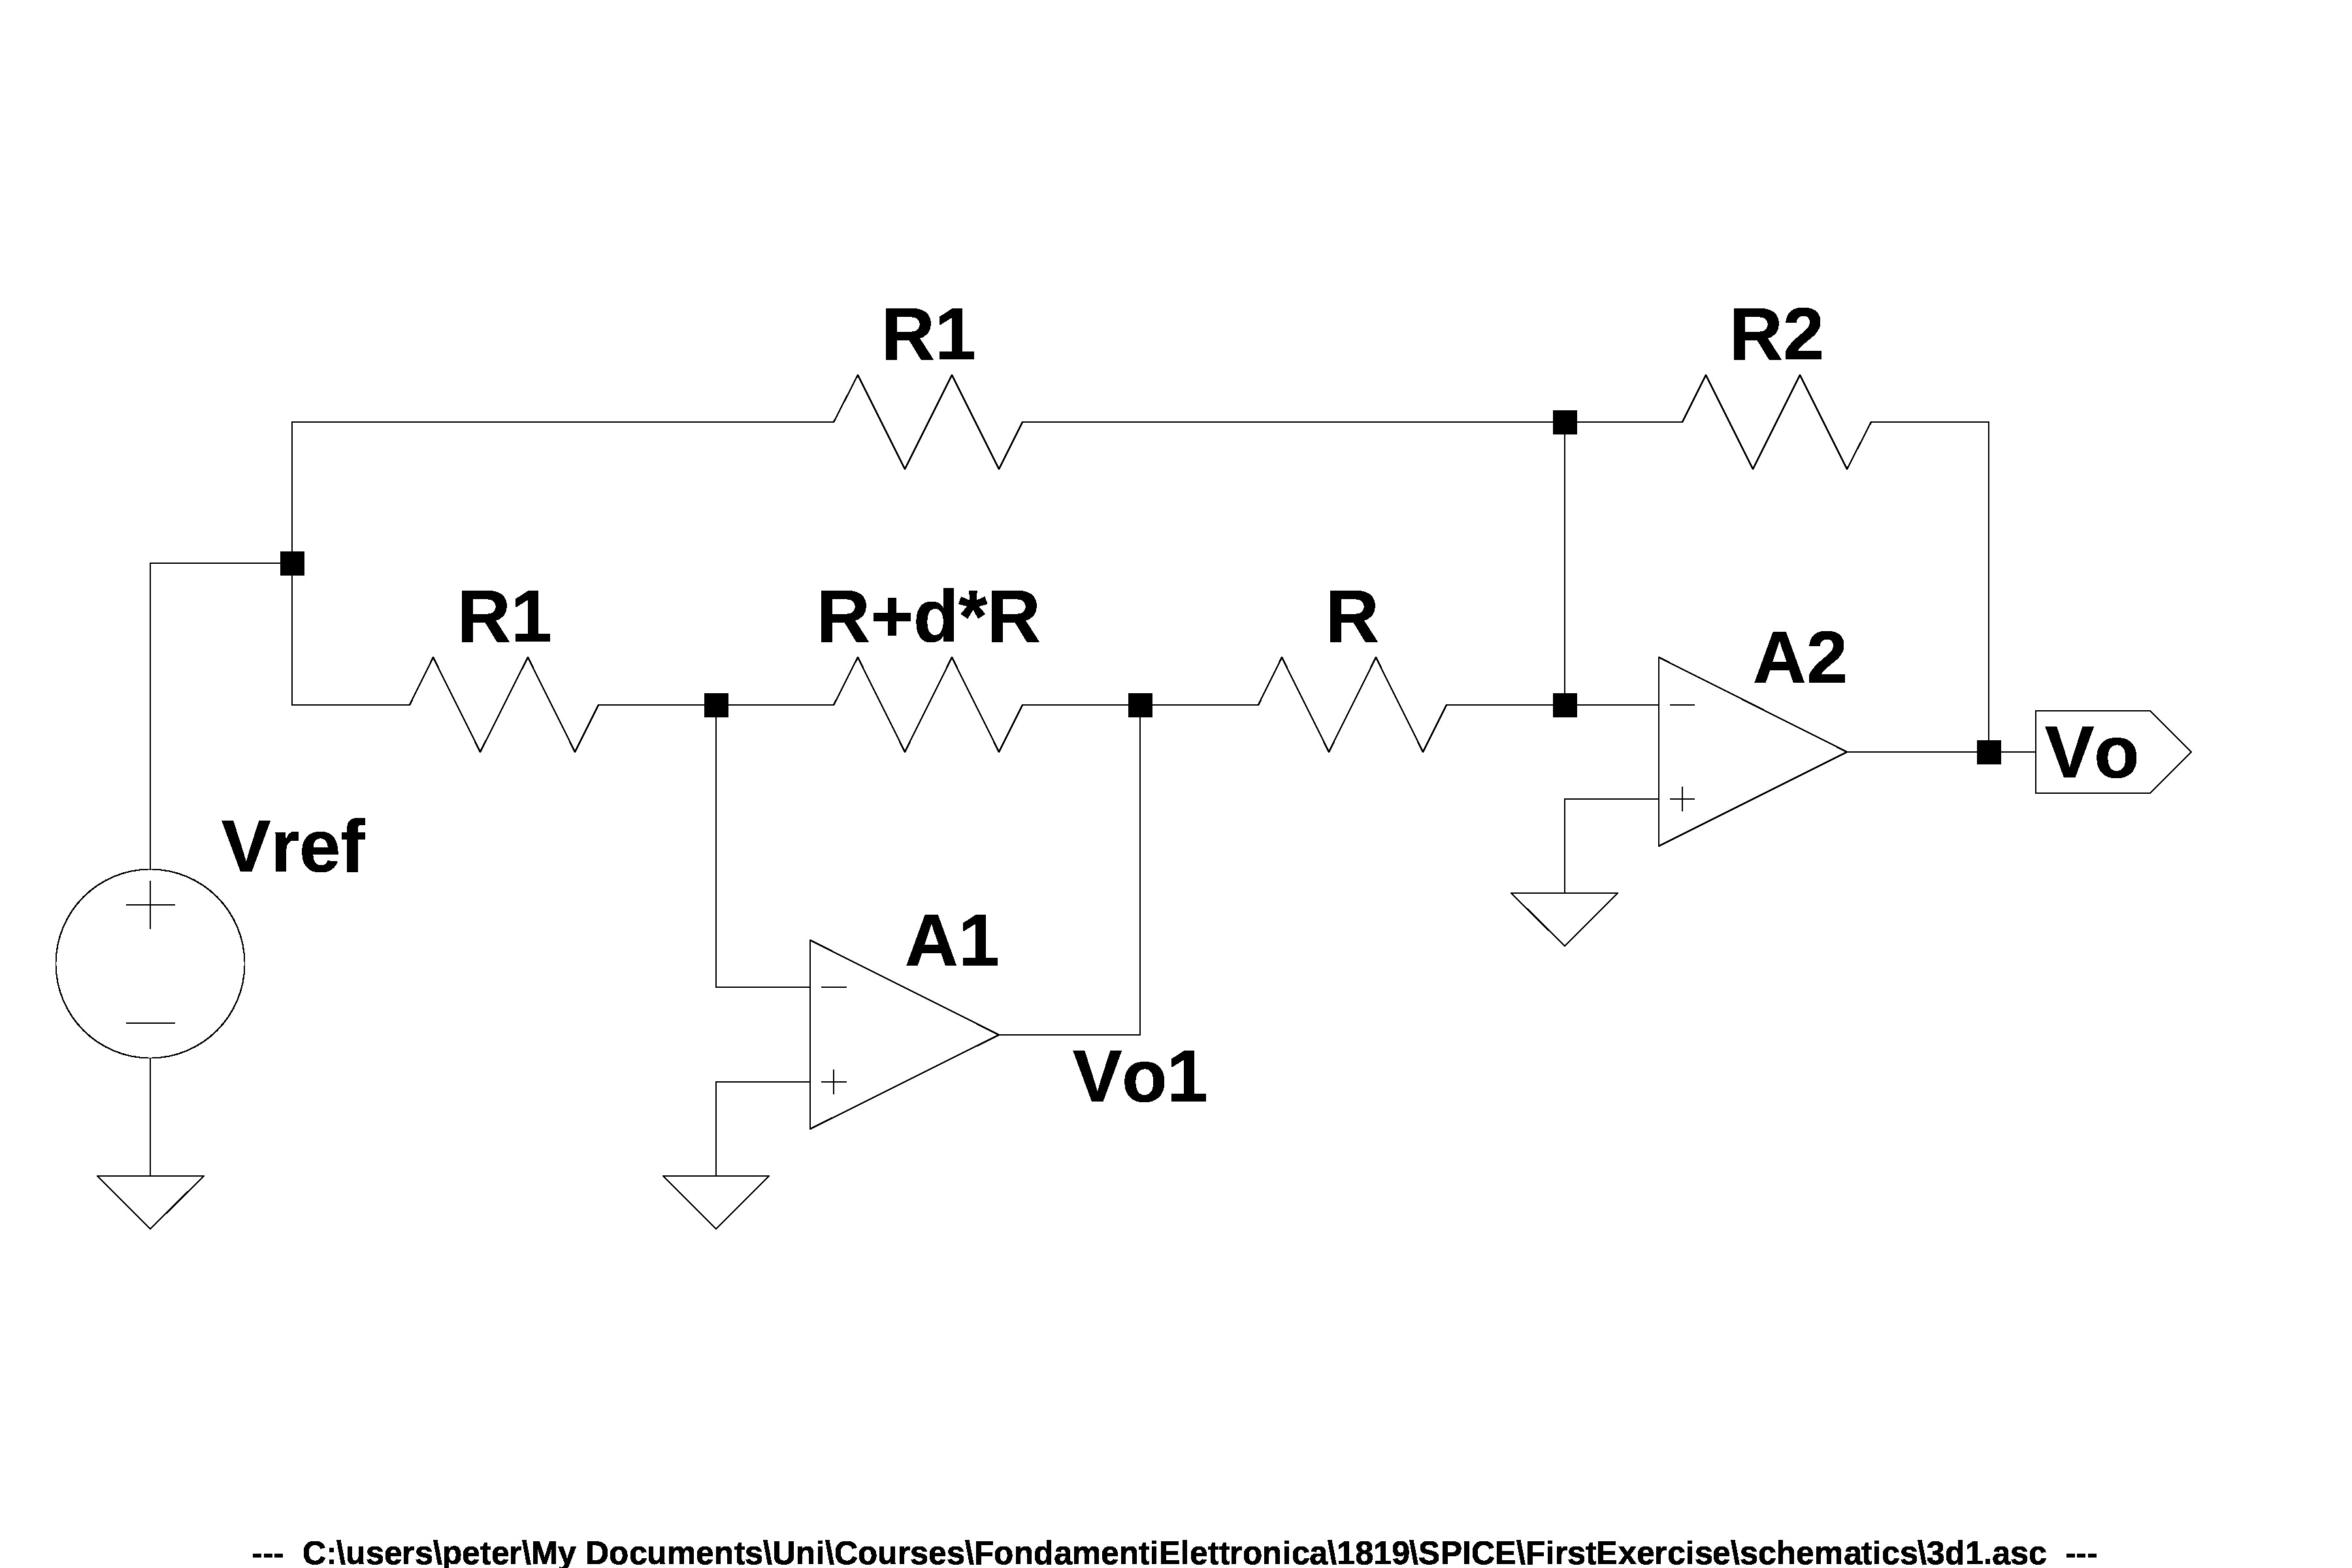
\includegraphics[width=12cm]{schematics/3d1.jpg}
  \caption{Front-end amplifier for resistive bridge with resistometric sensor}
  \label{3d1schematics}
\end{figure}

\section{Output voltage - $V_o$}

\begin{equation} \label{I_R1}
  I_{R_1} = \frac{V_{ref}}{R_1} = - I_{R+\delta R}
\end{equation}

\begin{equation} \label{V_o1}
  V_{o_1} = (R+\delta R) \cdot I_{R+\delta R}
  = (R+\delta R) \cdot \frac{V_{ref}}{R_1}
  = V_{ref} \cdot \frac{R+\delta R}{R_1}
\end{equation}

\begin{equation} \label{I_R}
  I_R = \frac{V_{o_1}}{R} = V_{ref} \cdot \frac{R+\delta R}{R_1R}
  = V_{ref} \cdot \frac{1+\delta}{R_1}
\end{equation}

\begin{equation} \label{I_R2}
  I_{R_2} = I_{R_1} + I_R
\end{equation}

\begin{align}
  V_o &= R_2 I_{R_2} = R_2 (I_{R_1} + I_R) \nonumber \\
  &= R_2 \left(- \frac{V_{ref}}{R_1} + V_{ref} \cdot \frac{1+\delta}{R_1} \right) \nonumber \\ 
  &= R_2 V_{ref} \left( \frac{-1+1+\delta}{R_1} \right) \nonumber \\
  &= V_{ref}\frac{R_2}{R_1}\delta \label{V_o}
\end{align}

\section{Defining $R_2$ and $R_1$}
Conditions:
\begin{equation} \label{eq:conditions3}
  \left\{
    \begin{array}{l}
      R_2 = \frac{1097752}{20}\Omega \\
      V_{ref} = 15V \\
      \frac{R_2}{R_1}V_{ref} = 20
    \end{array}
  \right.
\end{equation}

\begin{equation} \label{eq:R2R1_3}
  \left\{
    \begin{array}{l}
      R_1 = 41.16570k\Omega \\
      R_2 = 54.88760k\Omega \\
      V_{ref} = 15V
    \end{array}
  \right.
\end{equation}

\section{Graph of the output voltage - $V_o$}

\begin{figure}[H]
  \centering
  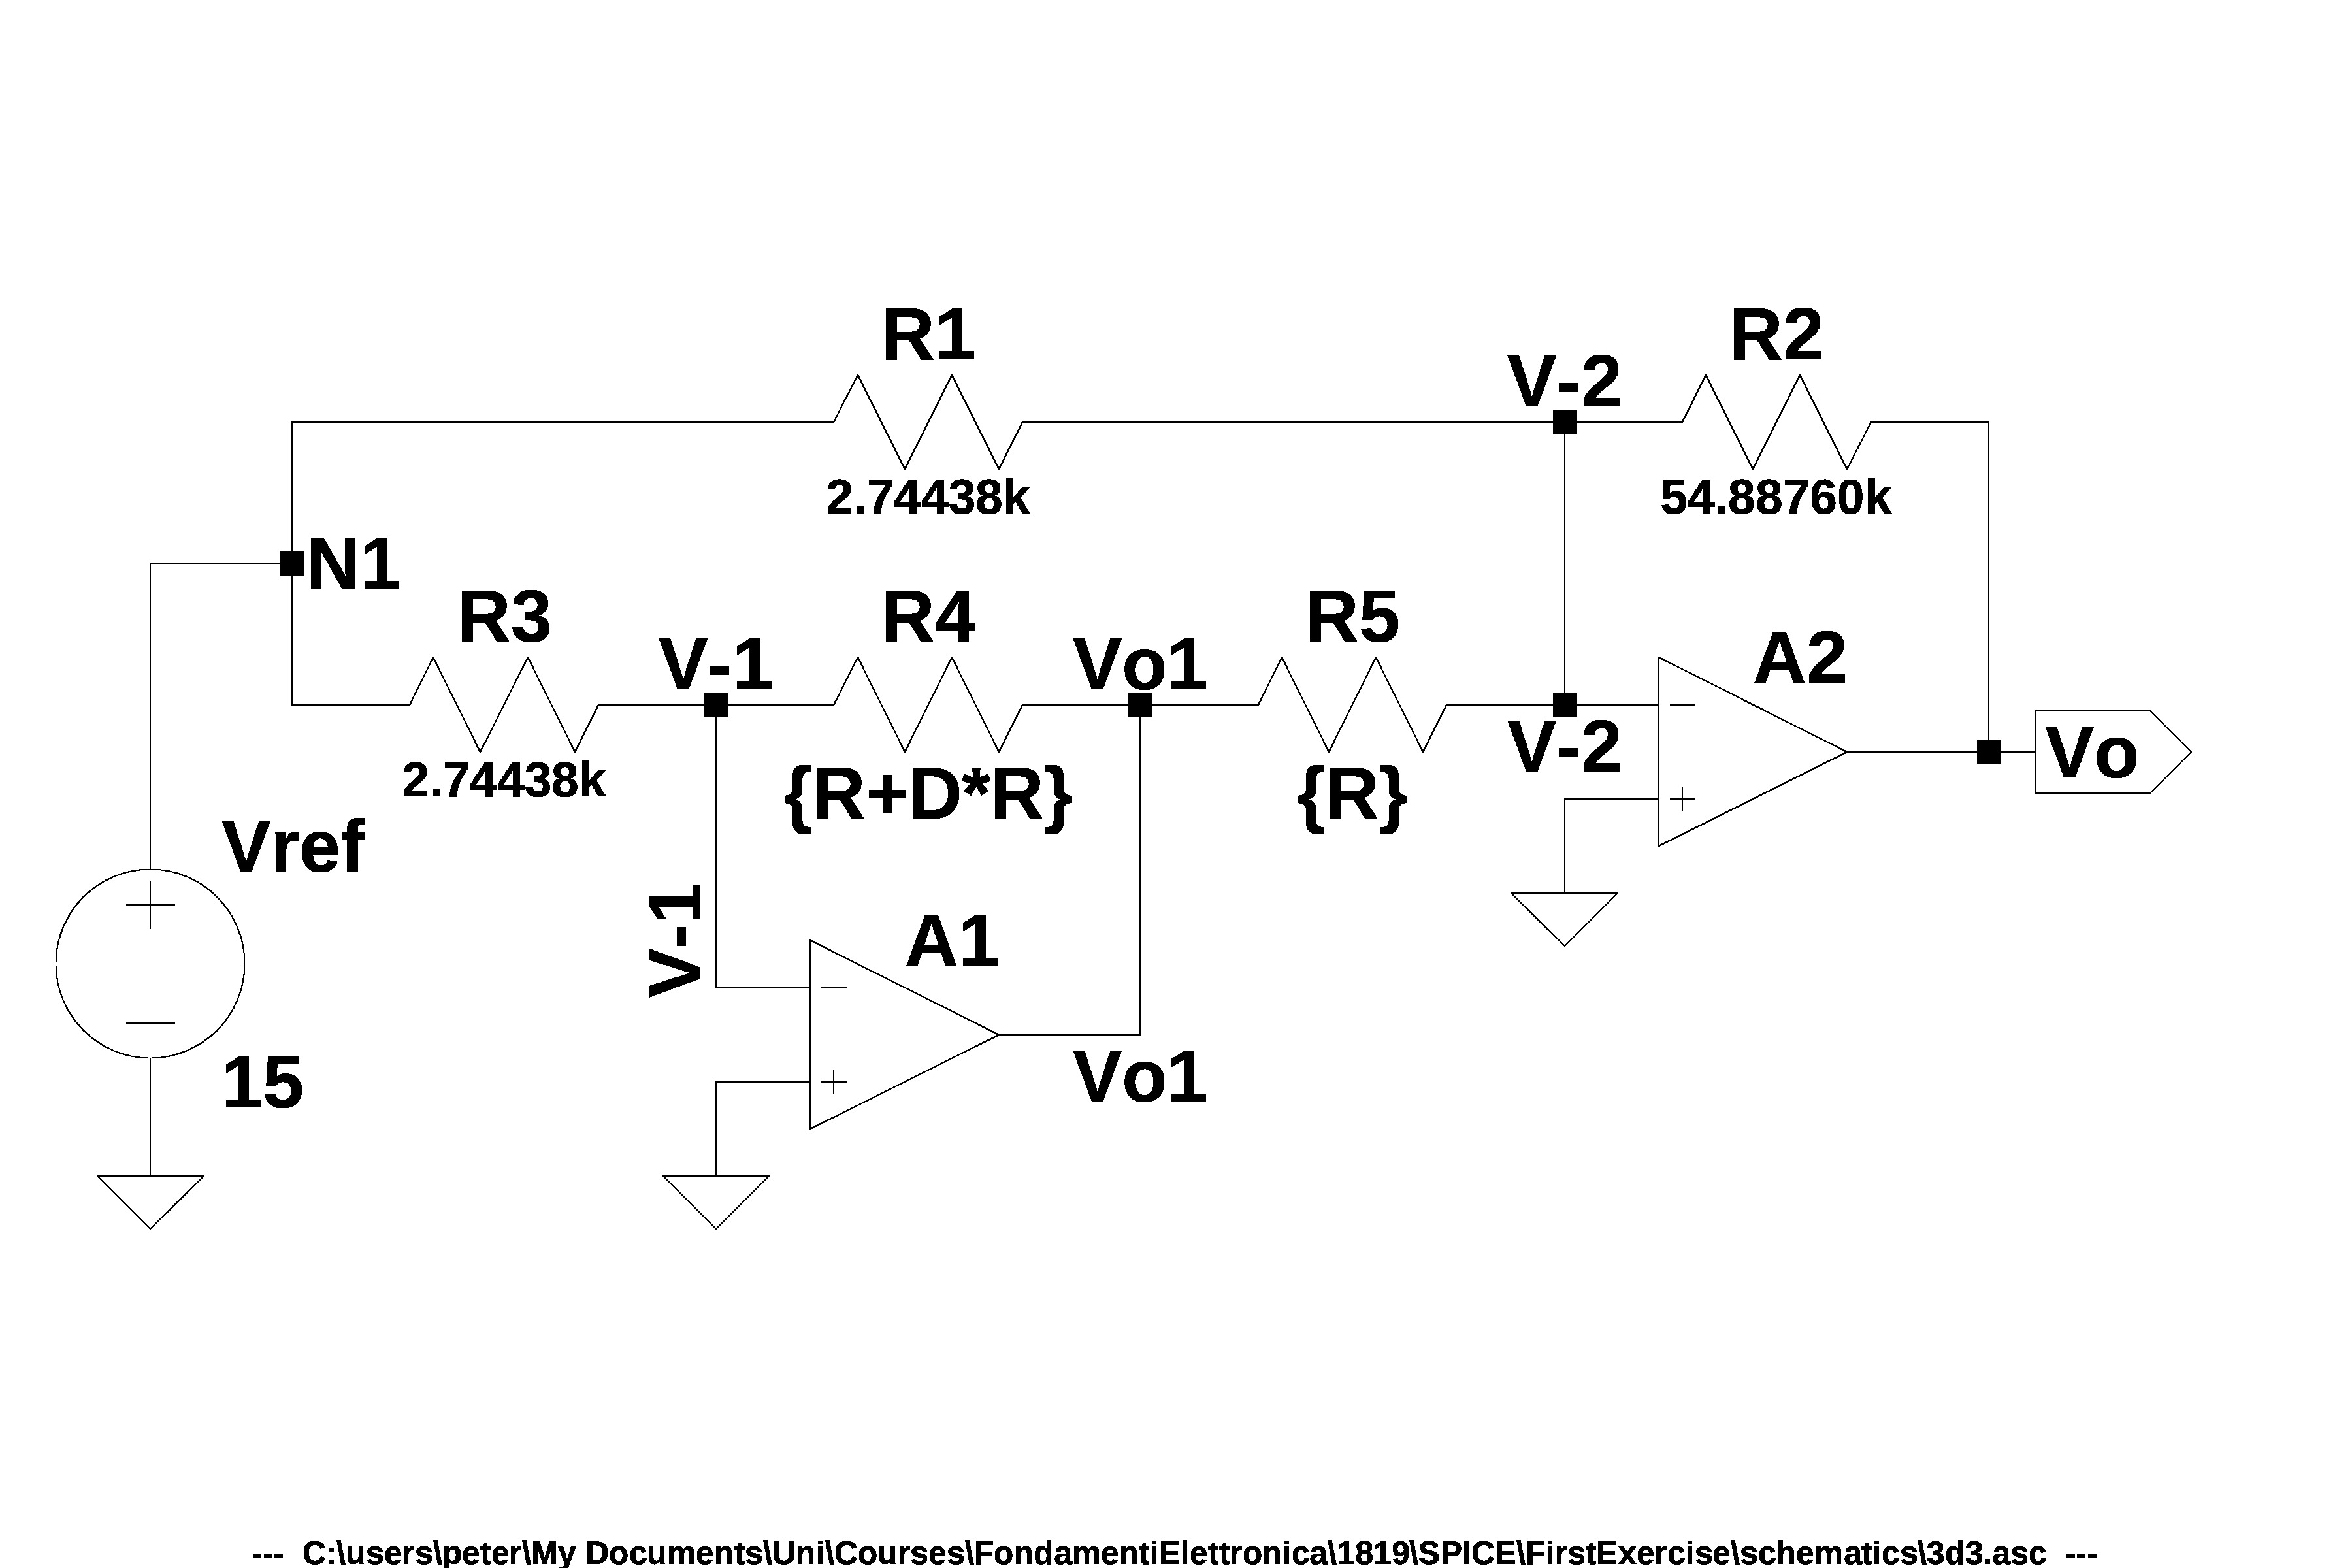
\includegraphics[width=12cm]{schematics/3d3.jpg}
  \caption{Front-end amplifier for resistive bridge with resistometric sensor - SPICE compatible schematics}
  \label{3d3schematics}
\end{figure}

\lstinputlisting{netlist/3d3.cir}

\begin{figure}[H]
  \centering
  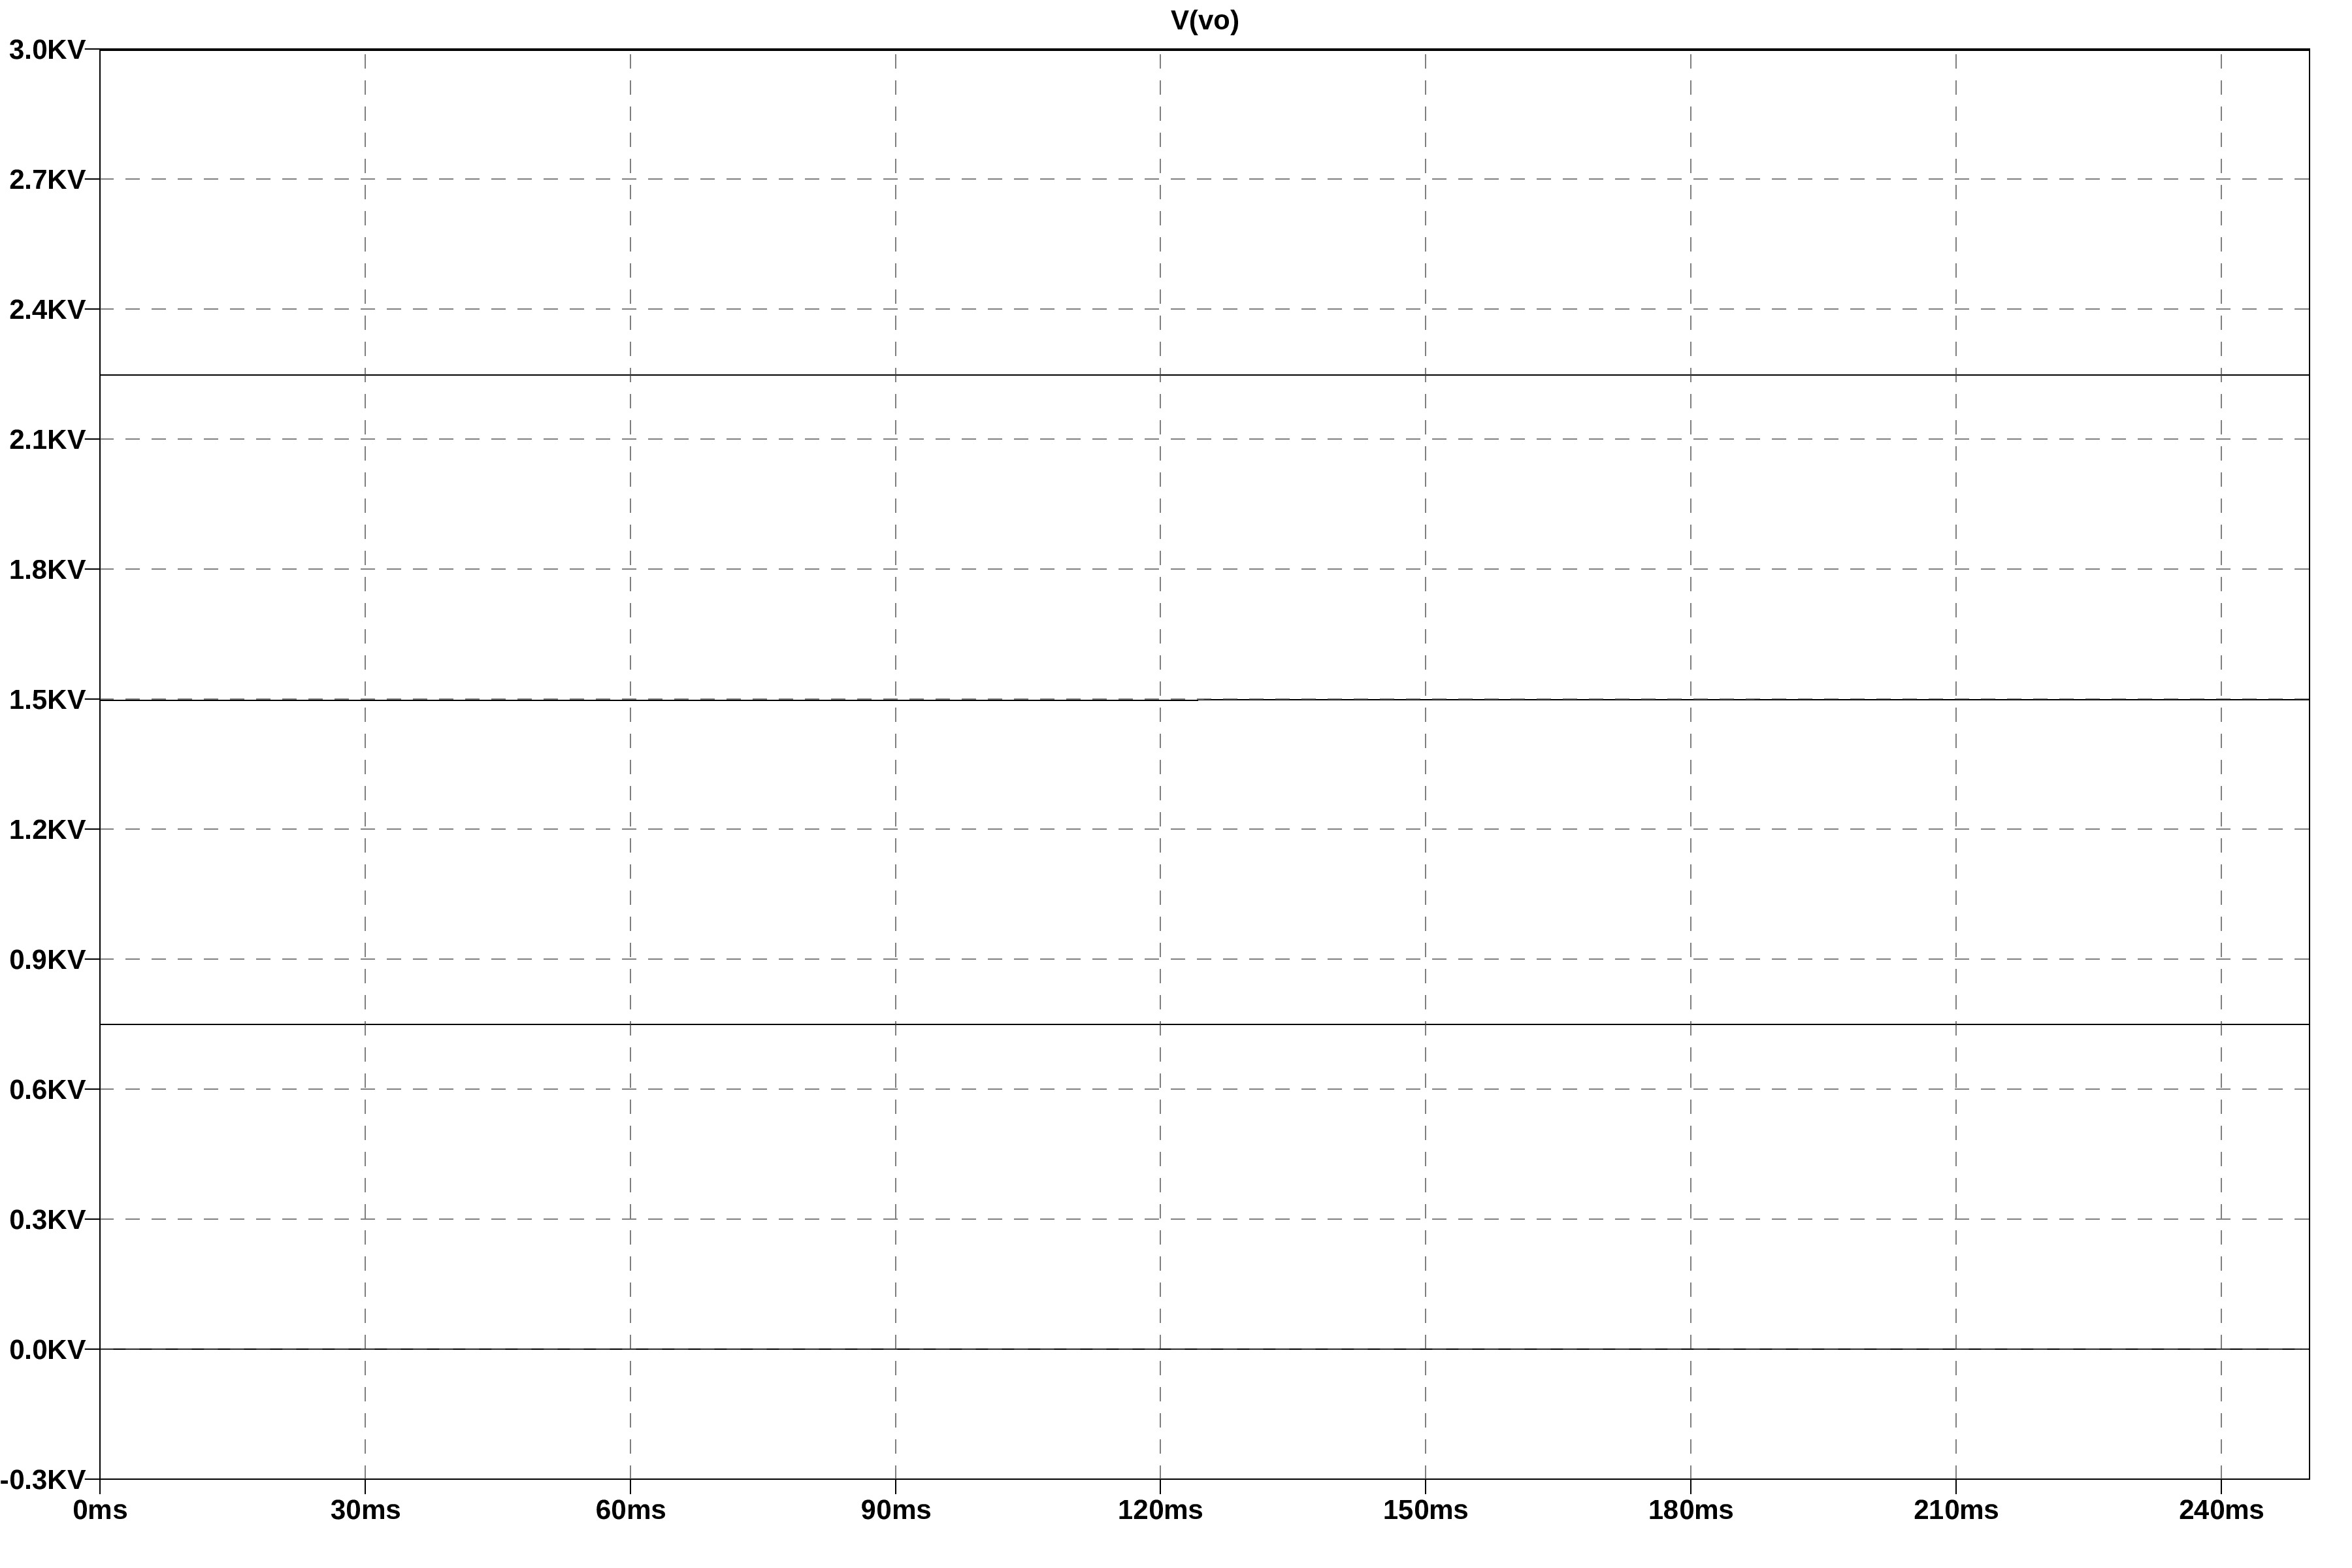
\includegraphics[width=14cm]{graph/3d3.jpg}
  \caption{Front-end amplifier for resistive bridge with resistometric sensor - $V_o$ with $R = 1k\Omega$ and $\delta = 0$, $\delta = 2.5$, $\delta = 5$ $\delta = 7.5$, $\delta = 10$}
  \label{3d3graph}
\end{figure}

\end{document}